%%%%%%%%%%%%%%%%%%%%%%%%%%%%%%%%%%%%%%%%%
% Design based on a template by Roberto and following the format of
% the xmipp tutorials. In turn, they seem to be based on a template
% from http://www.latextemplates.com
%%%%%%%%%%%%%%%%%%%%%%%%%%%%%%%%%%%%%%%%%

%----------------------------------------------------------------------------------------
%	PACKAGES AND OTHER DOCUMENT CONFIGURATIONS
%----------------------------------------------------------------------------------------

\documentclass[12pt, draft]{article} % Default font size is 12pt, it can be changed here
\usepackage[english]{babel}
\usepackage[utf8]{inputenc}
\usepackage{listings} % To include source code
\usepackage{caption}
\usepackage[htt]{hyphenat}
\usepackage{geometry} % Required to change the page size to A4
%\geometry{a4paper} % Set the page size to be A4 as opposed to the default US Letter
\usepackage{framed}
\usepackage{url}
\usepackage{graphicx} % Required for including pictures
\usepackage{natbib}
\usepackage{float} % Allows putting an [H] in \begin{figure} to specify the exact location of the figure
\usepackage{hyperref}
\usepackage{menukeys}
\usepackage{array}
\usepackage{fancyhdr}
\usepackage{marvosym}%smileys\Smiley{} \Frowny{}
\usepackage{etoolbox}
\usepackage{listings}
\usepackage{makecell}
\usepackage{marginnote}
\usepackage{soul}
\usepackage[toc,page]{appendix}
\usepackage{caption}
\usepackage{menukeys}
\usepackage{fancybox,framed}
\usepackage{xspace}
\usepackage{rotating}
\def\scipion{\textit{Scipion}\xspace}
\newcommand{\ffigure}[1]{{Fig. {\ref{#1}}}\xspace}
\newcommand{\ttable}[1]{{Table. {\ref{#1}}}\xspace}
\newcommand{\scommand}[1]{{{\keys{#1}}}\xspace}
\newcommand{\ccmask}{CC\textsubscript{MASK}\xspace}

\sethlcolor{yellow}

%\renewcommand{\hl}[1]{#1}
%pdflatex -jobname=students '\def\student{}\input{main}'
%pdflatex -jobname=teachers '\def\teachers{}\input{main}'
%  \ifdef{\teachers}
%  {Content for teachers}
%  {Content for students} 
\newcommand{\ttt}[1]{\texttt{#1}}
\newcommand{\iii}[1]{\textit{#1}}
\newcommand{\ra}{$\rightarrow$}
\pagestyle{fancy}
\fancyhf{}
\fancyhead[RO]{{Model Building}}
\fancyhead[LO]{Scipion}
%\fancyhead[RO]{{\leftmark}}
\fancyfoot[RO]{\thepage}

\linespread{1.2} % Line spacing

%\setlength\parindent{0pt} % Uncomment to remove all indentation from paragraphs

\newenvironment{command}{\tt\begin{quote}}{\end{quote}}
\newcommand{\comm}[1]{\texttt{#1}}

\newcommand{\imgfig}[3]{\begin{figure}[H]\centering \
\includegraphics[scale=#2]{images/#1} \caption{#3} \end{figure}}

\newcommand{\proto}[1]{\textit{\textbf{#1}}}
\newcommand{\popt}[1]{\textit{#1}}
\newcommand{\pval}[1]{\texttt{#1}}

\newcommand\tstrut{\rule{0pt}{2.4ex}}
\newcommand\bstrut{\rule[-1.0ex]{0pt}{0pt}}

\def \humanAdenoMap {7034}%5172

\begin{document}

%----------------------------------------------------------------------------------------
%	TITLE PAGE
%----------------------------------------------------------------------------------------

\begin{titlepage}

% New command for horizontal lines. Change thickness here.
\newcommand{\HRule}{\rule{\linewidth}{0.5mm}}

\center % Center everything on the page

\includegraphics{images/scipion_logo.png}

{\large Scipion Tutorial Series}\\[1.0cm]

\textsc{\LARGE National Center for Biotechnology}\\[0.5cm]
\textsc{\Large Biocomputing Unit}\\[0.15cm]

\HRule\\[0.4cm]
{ \huge \bfseries Model Building Basic}\\ % Title of your document
\HRule \\[0.5cm]
%{\large \today}\\[3cbum] % Date, change the \today to a set date if you want to be precise
\begin{center}
\includegraphics[width=0.70\textwidth]{{images/aadensity}.png}\\
Density for amino acid side chains from an experimental electron density map at 1.5 \AA~resolution (http://people.mbi.ucla.edu/sawaya/m230d/Modelbuilding/modelbuilding.html)\end{center}

%\vfill % Fill the rest of the page with whitespace
%\begin{minipage}{0.4\textwidth}
\begin{flushright}
 \large
%\emph{Author:}\\
  \textsc{Roberto Marabini AND Marta Martínez} % Your name
\end{flushright}
%\end{minipage}

\end{titlepage}


%----------------------------------------------------------------------------------------
%	OBJETIVOS
%----------------------------------------------------------------------------------------


\subsection*{Intended audience}
The recent rapid development of single-particle electron cryo-microscopy (cryo-EM) allows structures to be solved by this method at almost atomic resolutions.  Providing a basic introduction to model building, this tutorial shows the initial workflow aimed at obtaining high-quality atomic models from cryo-EM data by using \scipion software framework. %tomography in  electron microscopy with special emphasis in basic image processing. The tutorial requires matlab but does not assume any programing skills. 


\subsection*{We'd like to hear from you}

We have tested and verified the different steps described in this demo
to the best of our knowledge, but since our programs are in continuous
development you may find inaccuracies and errors in this text. Please
let us know about any errors, as well as your suggestions for
future editions, by writing to
\href{mailto:scipion@cnb.csic.es}{scipion@cnb.csic.es}.


\subsection*{Requirements}

This tutorial requires, in addition to \scipion,  the modeling system $USCF Chimera$ (\url{https://www.cgl.ucsf.edu/chimera/download.html}), the \textit{CCP4 suite} (\url{http://www.ccp4.ac.uk/download/#os=linux}) including $refmac$ and $coot$, the \textit{PHENIX suite} (\url{https://www.phenix-online.org/download/}) and \textit{PowerFit} application (\url{https://github.com/haddocking/powerfit}). Basic knowledge of $USCF Chimera$ and \scipion is assumed. Warning: old versions of $refmac$ are not suitable for EM data.

\newpage


%----------------------------------------------------------------------------------------
%	TABLE OF CONTENTS
%----------------------------------------------------------------------------------------

\tableofcontents % Include a table of contents

\newpage % Begins on a new page instead of on the same page as the table of contents


\section{Introduction to image processing}

\subsection*{Definition}
 Image processing is a structure determination technique that allows to get the 3D density map from a set of cryo-EM images of a particular macromolecule. Although different structural approaches can be followed to analyze the structures of macromolecules, this tutorial focuses on cryo-EM single particle analysis (SPA).  Fortunately, cryo-EM SPA is undergoing in this decade a resolution revolution that has allowed the structures of macromolecules to be solved at near-atomic resolution. 


 \subsection*{ Image processing workflow}
 
 The set of successive tasks aimed to get the 3D density map is known as image processing workflow. Main steps of the general workflow are detailed from top (movies) to bottom (refined volume) in the \ffigure{fig:image_processing_workflow}. Some of the tools required to perform the respective tasks are detailed in a non-exhaustive way on the right side of the Figure. All these methods have been integrated in \scipion to facilitate interoperability among different software packages, data tracking and reproducibility of results. 
 
 \begin{figure}[H]
 \centering
 \captionsetup{width=.8\linewidth}  \includegraphics[width=0.55\textwidth]
  {{images/Fig1.pdf}}
  \caption{General image processing workflow for SPA \citep{scipion2016}. }
  \label{fig:image_processing_workflow}
  \end{figure} 
 
 The workflow considers as input the movie frames generated by the microscope. These movies should be global or locally aligned before computing the CTF of individual micrographs. \scipion allows to compare different CTF values obtained with distinct algorithms using the CTF consensus protocol. Once the CTF has been corrected, we are ready to extract individual particles of each micrograph by using different protocols of particle picking. As in the case of the CTF, we can retrieve the coordinates of each particle using different protocols of manual and automatic picking, and finally, estimate the agreement between all those methods through a consensus picking protocol. The screened particles are used for further processing. The next step involves the 2D classification of the individual selected particles. 2D classes derived from the last procedure contribute to generate the initial 3D map. The last part of the workflow includes 3D classification and 3D refinement tasks in order to iterative refine the initial 3D map.
 
 In this tutorial, we show all above mentioned processes of 3DEM processing, as well as the necessary tools to accomplish them, illustrating the combination of different EM software packages in \scipion. 

 

 

  


\section{Problem to solve: Apoferritin}

Ferritins are iron storage metalloproteins ubiquitously distributed among living organisms. These proteins are involved in iron metabolism in many different types of cells, and play a relevant dual role both in iron detoxification and iron reserve. The ferritin's architecture, similar to a spherical shell, is highly conserved in bacteria, plants and animals, and it allows to accumulate high amounts of Fe(III) atoms (up to 4000 per molecule). \\

The highly stable iron-free shell is known as apoferritin. Mammalian apoferritins are heteromeric molecules, constituted by 24 monomers structurally equivalent that surround the central cavity. Among these monomers, variable proportions of two types of subunits with different properties, H (heavy) and L (light), can be found. The tissues involved in iron storage contain higher proportion of L chains, whereas the tissues that require higher protection against oxidation, such as heart or brain, have a higher content of H chains. Unlike L chains, H chains display ferroxidase catalytic activity, necessary to oxidize Fe(II) to Fe(III). Concerning the structure of each subunit, it is constituted by 4 long helices, a fifth smaller helix and an additional extended loop. The dinuclear iron site, or ferroxidase site, is located in the center of the four helix bundle.\\

This tutorial will guide us in the building process of the mouse apoferritin 3D map using the \scipion framework (\ffigure{fig:workflow_pdf}). As starting input data, we are going to use the \ttt{EMPIAR ID: 10248} data, obtained from mouse heavy chain apoferritin. This cryo-EM data allowed to generate the 3D map \ttt{EMD-9865} at 1.54 \AA\ resolution \citep{hamaguchi2019}. The most recent atomic structure of mouse apoferritin, homo 24-mer of ferritin heavy chain with octahedral symmetry, was also obtained from cryo\-EM data at 1.84 \AA\ (\ttt{PDB ID: 6S61}). The 24 monomers of this metal binding protein are ligated to 6 Fe(III) and 24 Zn(II) ions.

\subsection*{Apoferritin processing workflow in \scipion}
\begin{figure}[H]
  \centering
  \captionsetup{width=.8\linewidth} 
  \includegraphics[width=0.95\textwidth]
  {images/workflow.pdf}
  \caption{Apoferritin processing workflow.}
  \label{fig:workflow_pdf}
  \end{figure}







\section{Input data description}

 \subsection*{Volume}
 \ttt{EMD-3488}, that can be downloaded from \ttt{PDBE} (\url{http://www.ebi.ac.uk/pdbe/entry/emdb/EMD-3488}). %This volume emulates any other volume that you might obtain experimentally and reconstruct by single particle analyis.
 
 \begin{figure}[H]
  \centering
  \captionsetup{width=.8\linewidth} 
  \includegraphics[width=0.95\textwidth]
  {{Images/Fig3}}
  \caption{Downloading the volume from \ttt{PDBE}.}
  \label{fig:PDBE}
  \end{figure}
  
  Once downloaded the volume, unpack it (command line: \ttt{gunzip emd-3488.map.gz}) and save it in your tutorial folder.
 
 \subsection*{Sequences}
 
 The sequences of \ttt{Hgb} $\alpha$ and $\beta$ subunits are included in \ttt{UniProtKB}. Accession numbers are \ttt{P69905} and \ttt{P68871}, respectively. In the following we show both sequences in fasta format:
 \begin{quote}
   \begin{verbatim}
>sp|P69905|HBA_HUMAN Hemoglobin subunit alpha
MVLSPADKTNVKAAWGKVGAHAGEYGAEALERMFLSFPTTKTYFPHFDLSHGSAQVKGHG
KKVADALTNAVAHVDDMPNALSALSDLHAHKLRVDPVNFKLLSHCLLVTLAAHLPAEFTP
AVHASLDKFLASVSTVLTSKYR

>sp|P68871|HBB_HUMAN Hemoglobin subunit beta
MVHLTPEEKSAVTALWGKVNVDEVGGEALGRLLVVYPWTQRFFESFGDLSTPDAVMGNPK
VKAHGKKVLGAFSDGLAHLDNLKGTFATLSELHCDKLHVDPENFRLLGNVLVCVLAHHFG
KEFTPPVQAAYQKVVAGVANALAHKYH
\end{verbatim}
 \end{quote}

 
 These protein sequences were determined by direct translation from the experimental sequence obtained from complementary \ttt{DNA (cDNA)}, i.e., \ttt{DNA} synthesized or retro-transcribed from messenger \ttt{RNA (mRNA)}. In this way, it is quite unlikely that these sequences included post-translational modifications. Although methionine is added with the translation \ttt{Met-tRNA} initiation factor, the removal of methionine aminoacid from the N-terminus of a polypeptide is a common post-translational modification. Since methionine appears at the N-terminal end of both proteins, we can predict that these are not the polypeptide mature forms and Methionine will be removed in the mature ones that are present in the atomic structures. 
 
 These two sequences can be retrieved from \ttt{UniProtKB} using \scipion\ \scommand{import sequence} protocol which allows direct download from the database.
 


\section{Import Input data}
Taking advantage of \scipion software framework, we are going to import the above indicated input data using protocols \scommand{import volumes} and  \scommand{import sequence}. Details about the parameters of these two protocols are shown in Appendices \ref{app:importVolume} and \ref{app:importSequence}, respectively. 

(Note: The notation \ttt{Fig. X (a)} means that the step is shown in figure number X and there will be an arrow labeled with ``a'' marking the region of interest.)

 \subsection*{Volume}
 First open the \scommand{import volumes} protocol (\ffigure{fig:import_volume} (1)), fill in the form and execute it (2), and finally you may visualize the volume (3). By default \chimera \citep{pettersen2004} is used for visualization (\ffigure{fig:chimera_visualization_volume}). It shows the 3D map and the $x$ (red), $y$ (yellow) and $z$ (blue) axes.  
 %  The C2 symmetry is shown, as well as the 45º turn of volume regarding the z axis (blue line).
 
 \begin{figure}[H]
  \centering 
  \captionsetup{width=.7\linewidth} 
  \includegraphics[width=0.80\textwidth]
  {Images/Fig4}
  \caption{Importing the volume in \scipion.}
  \label{fig:import_volume}
  \end{figure}
  
 \begin{figure}[H]
  \centering 
  \captionsetup{width=.7\linewidth} 
  \includegraphics[width=0.80\textwidth]
  {Images/Fig5}
  \caption{Volume visualized with \chimera.}
  \label{fig:chimera_visualization_volume}
  \end{figure}
 
 \subsection*{Sequences}
 
 The sequences of \ttt{Hgb} $\alpha$ and $\beta$ subunits will be independently downloaded from \ttt{UniprotKB}. First of all, open the form of \scommand{import sequence} protocol (\ffigure{fig:import_sequence} (1)), then complete the form to download \ttt{HBA\_HUMAN} protein with \ttt{UniProtKB} accession code \ttt{P69905}, execute the process (2), and finally visualize the sequence (3) in a text editor. The sequence will appear in fasta format as it has been written above. Follow the same protocol to download \ttt{HBB\_HUMAN} with accession code \ttt{P68871}.
 
 \begin{figure}[H]
  \centering 
  \captionsetup{width=.7\linewidth} 
  \includegraphics[width=0.80\textwidth]
  {Images/Fig6}
  \caption{Importing a \ttt{UniProtKB} sequence in \scipion.}
  \label{fig:import_sequence}
  \end{figure}
 
\section{3D Map preprocessing}
\ffigure{fig:scipion_workflow_import_2} shows the \scipion workflow that we are going to detail in this section.

 \begin{figure}[H]
  \centering 
  \captionsetup{width=.9\linewidth} 
  \includegraphics[width=0.95\textwidth]
  {Images/Fig62}
  \caption{\scipion framework detailing the workflow generated after 3D map preprocessing.}
  \label{fig:scipion_workflow_import_2}
  \end{figure}

\subsection*{Map sharpening}
As we have indicated before, since map sharpening contributes to increase  signal at medium/high resolution, we recommend to perform this map preprocessing step before tracing the atomic model of cryo-EM  3D maps \citep{ramirez2018}.  To accomplish this task a couple of automatic alternatives are available in \scipion:  a) local sharpening method independent of initial model, based on local resolution estimation  (\scommand{xmipp3 - localdeblur sharpening} \citep{ramirez2018} (Appendix \ref{app:localDeblurSharpening})), b) deep learning-based sharpening approach (\scommand{xmipp3 - deepEMhancer} \citep{Sanchez-Garcia2020.06.12.148296} (Appendix \ref{app:deepEMhancerSharpening})). 

\subsubsection*{a) Sharpening with $LocalDeblur$}
Since $LocalDeblur$ takes advantage of map local resolution to increase the signal, we have to compute this local resolution as first step to apply the $LocalDeblur$ sharpening method.  Although different algorithms could be used to compute local resolution, we have selected $MonoRes$ \citep{vilas2018}, implemented in \scipion in the protocol \scommand{xmipp3 - local MonoRes}  (Appendix \ref{app:localMonoRes}).\\ 
Since a map binary mask has to be included as a parameter in this protocol, we will build a mask by using the \scipion protocol \scommand{xmipp3 - create 3d mask} (Appendix \ref{app:create3DMask}) as starting step in the local resolution estimation process. Open the protocol form (\ffigure{fig:create3Dmask_1} (1)) and fill in the tap \ttt{Mask generation} (2) with the input volume (3) and the density threshold (4). By default, the level value observed in \chimera main  graphics window (\ffigure{fig:chimera_visualization_volume}) \ttt{Tools -> Volume Data -> Volume Viewer -> Level} can be selected as threshold. In the \ttt{Postprocessing} tap (\ffigure{fig:create3Dmask_1} (5)), select \ttt{Yes} in \ttt{Apply morphological operation} (6) and maintain the rest of options by default. After executing this protocol (\ffigure{fig:create3Dmask_1} (7)), the morphology of the mask generated can be checked in slices by clicking \ttt{Analyze Results} (8).

 
 \begin{figure}[H]
  \centering 
  \captionsetup{width=.9\linewidth} 
  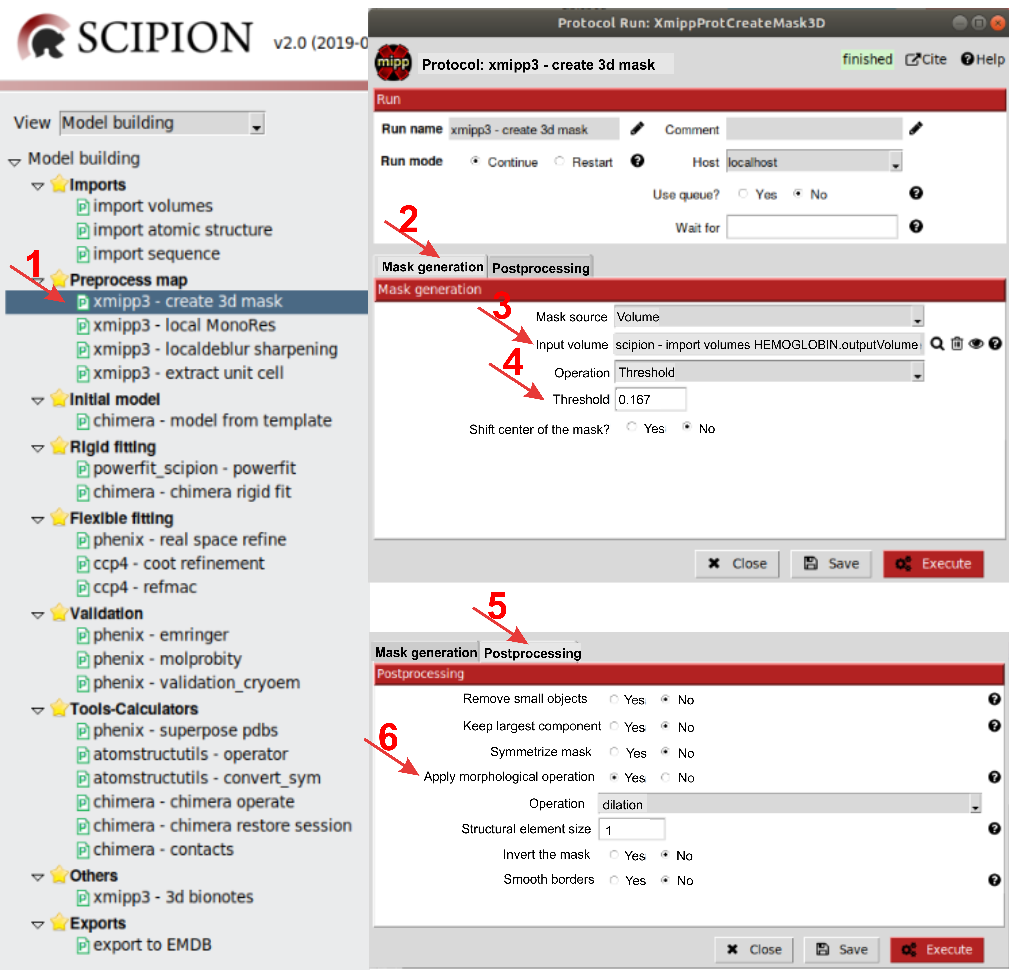
\includegraphics[width=0.95\textwidth]
  {Images/Fig53}
  \caption{Filling in the protocol to create a mask of the initial volume.}
  \label{fig:create3Dmask_1}
  \end{figure}
 
 $ShowJ$, the default \scipion viewer, allows visualize the mask with shape similar to the starting volume (\ffigure{fig:create3Dmask_2}).

 \begin{figure}[H]
  \centering 
  \captionsetup{width=.7\linewidth} 
  \includegraphics[width=0.60\textwidth]
  {Images/Fig54}
  \caption{Visualizing the mask of the initial volume.}
  \label{fig:create3Dmask_2}
  \end{figure}
  
\ttt{NOTE}: In case you would like to use a previous computed mask, you can do it simply by importing it using the protocol \scommand{import mask} (Appendix \ref{app:importMask}).\\
  
Once the mask of the starting map has been created, the protocol of \scommand{xmipp3 - local MonoRes} can be completed to get the estimation of local resolution. Open the protocol (\ffigure{fig:localMonoRes_1} (1)) and include the starting map (2), as well as the binary mask (3). Finally, based on the map resolution (3.2 \AA), select the default resolution range between \ttt{0.0} and \ttt{6.0} \AA (4). 

\begin{figure}[H]
  \centering 
  \captionsetup{width=.9\linewidth} 
  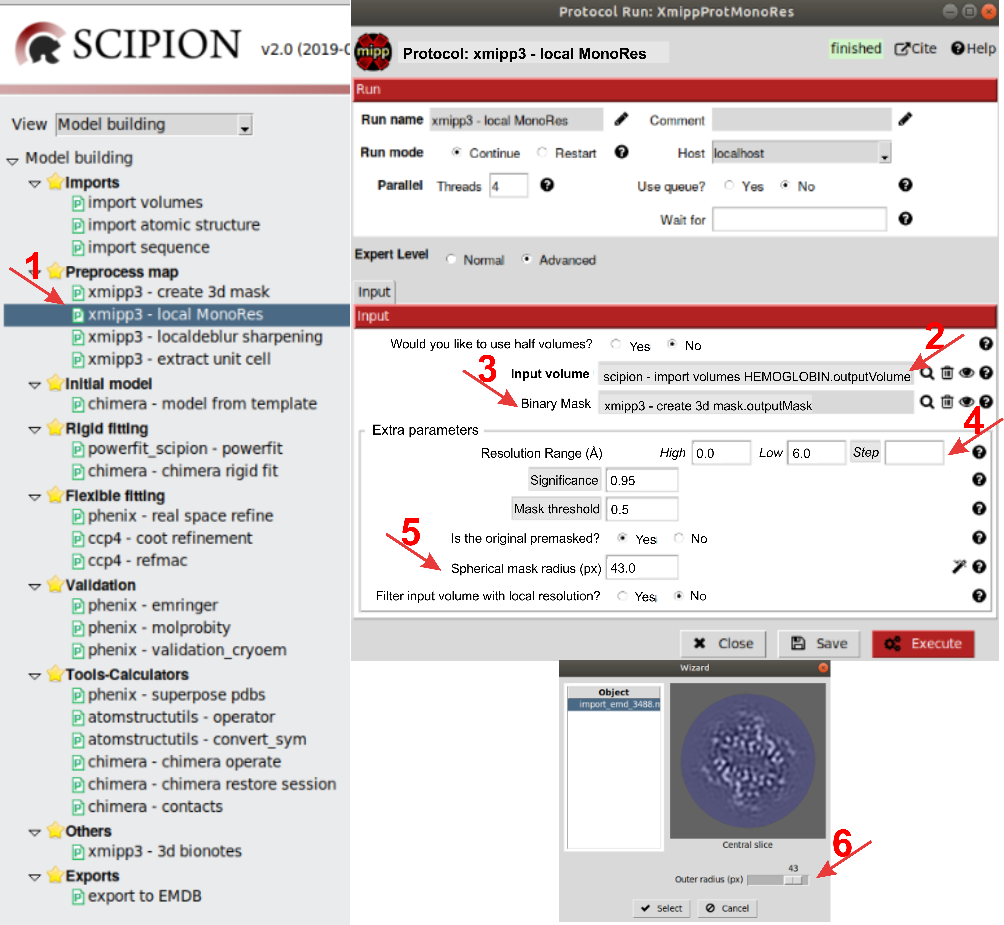
\includegraphics[width=1\textwidth]
  {Images/Fig55}
  \caption{Completing the protocol to estimate the local resolution of the \ttt{metHgb} map.}
  \label{fig:localMonoRes_1}
  \end{figure}
  
Execute this protocol (\ffigure{fig:localMonoRes_1} (5)) and analyze the results (6). The menu of results (\ffigure{fig:localMonoRes_2} (A)), among other views, shows the histogram of local resolutions (1) and the resolution map in \chimera (2). The histogram of resolutions, which displays the number of map voxels showing a certain resolution, allows to conclude that the majority of voxels evidence a resolution between 3.2 and 3.5 \AA, quite close to the published map resolution (3.2 \AA).The resolution map shown by \chimera details the resolution of each voxel (\ffigure{fig:localMonoRes_3}). The bar on the left indicates the color code for resolution values.

\begin{figure}[H]
  \centering 
  \captionsetup{width=.7\linewidth} 
  \includegraphics[width=0.80\textwidth]
  {Images/Fig56}
  \caption{\scommand{xmipp3 - local MonoRes} menu of results (A) and histogram of resolutions (B).}
  \label{fig:localMonoRes_2}
  \end{figure}
  
\begin{figure}[H]
  \centering 
  \captionsetup{width=.7\linewidth} 
  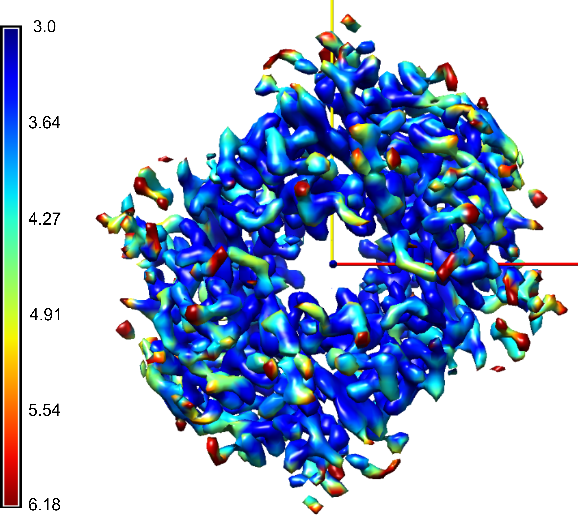
\includegraphics[width=0.70\textwidth]
  {Images/Fig57}
  \caption{Resolution map in \chimera.}
  \label{fig:localMonoRes_3}
  \end{figure}
  
Local resolution values of the input map allow to compute the sharpened map by the \scommand{xmipp3 - localdeblur sharpening} protocol, which implements an iterative steepest descent method that not requires initial model. To accomplish this step, open the protocol (\ffigure{fig:localdeblur_1} (1)) and include the starting map (2) and the map of resolution values (3), maintaining the default values for the rest of parameters (4, 5). 

\begin{figure}[H]
  \centering 
  \captionsetup{width=.9\linewidth} 
  \includegraphics[width=1\textwidth]
  {Images/Fig58}
  \caption{Filling in the protocol to compute the sharpened map.}
  \label{fig:localdeblur_1}
  \end{figure}
  
After two iterations, the sharpening algorithm reached the convergence criterion, $i.e.$ a difference between two successive iterations lower than 1 \%, and stopped. The two maps obtained in the respective iterations can be observed with $ShowJ$ by clicking the black arrow shown in \ffigure{fig:localdeblur_1} (7) with the right mouse botton and selecting \ttt{Open with DataViewer}. Resulting map for each iteration will be shown, as indicated in \ffigure{fig:localdeblur_2}.  Visualization in \chimera is also possible selecting \ttt{Open with ChimeraX} in the menu option \ttt{File} (\ffigure{fig:localdeblur_2} (1)). 

\begin{figure}[H]
  \centering 
  \captionsetup{width=.7\linewidth} 
  \includegraphics[width=0.65\textwidth]
  {Images/Fig59}
  \caption{Sharpened maps generated after two iterations.}
  \label{fig:localdeblur_2}
  \end{figure}
  
Additionally, by clicking \ttt{Analyze Results} (\ffigure{fig:localdeblur_1} (6)) the sharpened map obtained after the second iteration, $i.e.$ the \ttt{last} map, can be also visualized and compared with the initial one in \chimera (\ffigure{fig:localdeblur_3}).


\begin{figure}[H]
  \centering 
  \captionsetup{width=.7\linewidth} 
  \includegraphics[width=0.65\textwidth]
  {Images/Fig64}
  \caption{$LocalDeblur$ \ttt{last} iteration sharpened map (yellow surface) and input map (grey mesh) in \chimera.}
  \label{fig:localdeblur_3}
  \end{figure}
 
\subsubsection*{b) Sharpening with $DeepEMhancer$}

$DeepEMhancer$ is an alternative automatic sharpening method based on deep learning (\citep{Sanchez-Garcia2020.06.12.148296}), implemented in \scipion in the protocol \scommand{xmipp3 - deepEMhancer} (Appendix \ref{app:deepEMhancerSharpening}). Open this protocol (\ffigure{fig:deepEMHancer_1} (1)) and complete it as indicated. Since only the refined map is available, we are not going to use half maps (2). Include your map (3), the type of normalization desired (4) and the deep learning mode to use (5), in this particular case \ttt{highRes} due to the map high resolution.

 
 \begin{figure}[H]
  \centering 
  \captionsetup{width=.9\linewidth} 
  \includegraphics[width=0.95\textwidth]
  {Images/Fig63}
  \caption{Filling in the protocol to generate a sharpened map with $DeepEMhancer$.}
  \label{fig:deepEMHancer_1}
  \end{figure}

After executing the protocol (\ffigure{fig:deepEMHancer_1} (6)), we can check the results (7). \chimera viewer will open and show the sharpened map compared with the initial one (\ffigure{fig:deepEMHancer_2}).

\begin{figure}[H]
  \centering 
  \captionsetup{width=.7\linewidth} 
  \includegraphics[width=0.65\textwidth]
  {Images/Fig65}
  \caption{$DeepEMhancer$ sharpened map (yellow surface) and input map (grey mesh) in \chimera.}
  \label{fig:deepEMHancer_2}
  \end{figure}
  
\subsection*{Comparison of maps}
Realize that at this point we have generated two optimized maps derived from the initial one. Additionally, some other maps could have been obtained using other map optimization methods. A comparison among them would be interesting to consider which one(s) of them should be used as input in next steps of modeling workflow. The ideal map for tracing the atomic structure should include as many details and connections as possible and, at the same time, preserve the density areas of the initial map. In other words, we can use the best sharpened map (with higher resolution) corroborating that it does not make up new densities, absent in the starting map. Nevertheless, choose ``the best'' sharpened map could be difficult sometimes, especially if the map is very big or there are some regions optimized in one of the sharpened maps and other areas optimized in the other one. In that case, you can use several maps at the same time, having all of them perfectly aligned according to the same origin of coordinates.

In the tiny example shown in this tutorial we are working with a high resolution map and there are almost no differences in resolution between the starting map and the two derived sharpened maps, although this is not usually the case in real life. In this quite uncommon case the initial unsharpened map would be enough to trace the atomic structure. However, in order to detail the method, the starting map and their two sharpened ones will be used simultaneously.




\subsection*{Extraction of the map asymmetric unit}
Since smaller volumes usually include lower number of individual structural elements, making easier fitting models in maps and simplifying modeling process, the part of the map chosen to work with will always be the smaller asymmetrical subunit of the starting loaded map, also known as asymmetric unit (ASU). The size of the ASU thus depends on the symmetry order of the initial volume. The higher the symmetry order, the smaller the ASU. The atomic structure of the whole volume will be obtained straight forward by simply repetition of the ASU structure according to the symmetry order. Then, the first step to simplify the complexity of the initial volume is extracting the ASU. This task can be accomplished by using the \scipion protocol \scommand{xmipp3 - extract unit cell} that extracts the geometrical ASU of the map (Appendix \ref{app:extractUnitCell}).\\

\ffigure{fig:extract_unit_cell} shows how to fill in this protocol form (1). Consider that in this particular case the protocol will be run three times, one with each map (the initial one and the two sharpened derived ones). Include each map in a protocol form parallel to that shown in \ffigure{fig:extract_unit_cell} (2). Since \ttt{metHgb} macromolecule shows symmetry C2, we have selected cyclic symmetry (Cn) as type of symmetry (3), and 2 as symmetry order (4). The angle offset selected (5) turns -45º around the Z axis the mask used to create the ASU. 
%Remark the relevance of including the offset in order to extract a unit cell able to reconstruct by symmetry the whole volume regarding the symmetry axes. 
The two wizards on the right (6, 7) help you to select the radii to delimit a fraction of the map comprised between the coordinate origin (inner radius 0.0) and the maximum radius (outer radius 50.0). The final extracted volume will be slightly higher than the ASU due to the expand factor 0.2 (8). % We use an expanded unit cell  to favor the modeling of each individual structure edges. 
The respective tutorial appendix \ref{app:extractUnitCell} includes a comprehensive explanation of the meaning of parameters. 

 \begin{figure}[H]
  \centering 
  \captionsetup{width=.9\linewidth} 
  \includegraphics[width=1\textwidth]
  {Images/Fig7}
  \caption{Extracting the map asymmetric unit (ASU).}
  \label{fig:extract_unit_cell}
  \end{figure}
  
After executing the protocol (\ffigure{fig:extract_unit_cell}(9)), the resulting expanded ASU can be observed (10) with \chimera (\ffigure{fig:chimera_visualization_unit_cell}). Note the additional expanded volume of the  ASU on the left side of the figure. The ASU itself, on the right side, constitutes the half volume. Since the total volume contains the structure of four proteins, we can anticipate that this smaller asymmetrical subunit of the initial volume contains two proteins, one $\alpha$ and one $\beta$ \ttt{metHbg} subunits. Then, the respective structures of these two proteins could be fitted in the map ASU simultaneously or in successive modeling workflow steps. 
  
 \begin{figure}[H]
  \centering 
  \captionsetup{width=.7\linewidth} 
  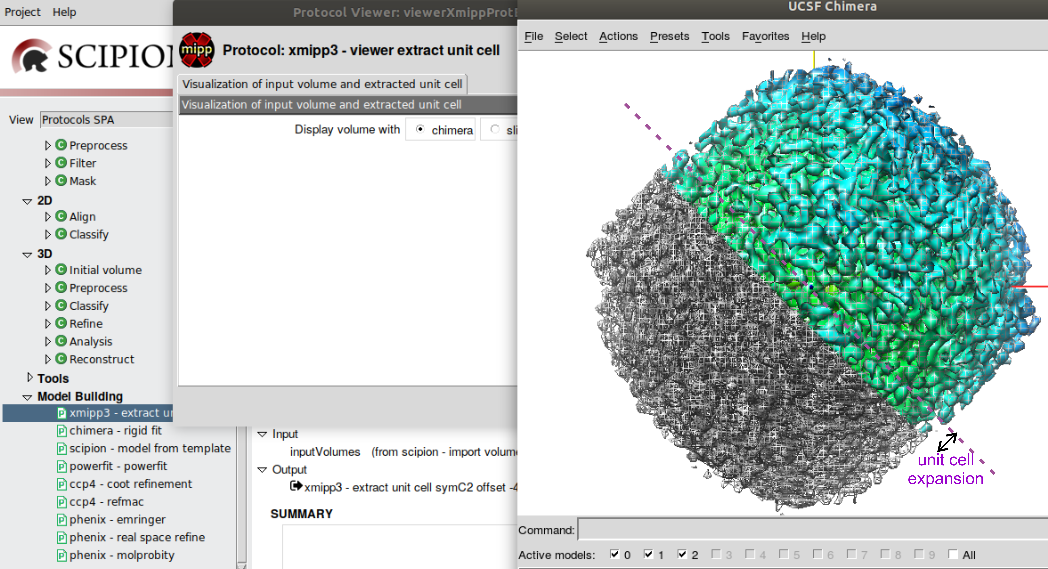
\includegraphics[width=0.80\textwidth]
  {Images/Fig8}
  \caption{Expanded ASU (yellow-green-blue) and initial volume (gray) visualized with $ChimeraX$. The purple broken line on the right delimits the ASU (right) and its expanded volume (left).}
  \label{fig:chimera_visualization_unit_cell}
  \end{figure}

\section{Structure Prediction by Sequence Homology. Searching for Homologues}
\label{sec:structurePrediction}
As we have mentioned above, in this tutorial we are going to use tools that allow to predict the atomic structure from sequence homology. 

Structure prediction by sequence homology only requires the sequence itself of the specimen that we would like to model, from now ahead the \iii{target sequence}, and the access to databases to seek structures or \iii{templates} of homologous molecules. The sequences of homologous molecules show statistically significant similarity because they share common ancestry. Since the sequence encodes the structural information, from high similar sequences necessarily follows high similar structures. Structures from the nearest homologous molecules will thus be preferred over remote relative ones. Remark that molecules containing several domains usually require independent searching for homologous templates of each domain. A small review about sequence similarity searching can be found in \citep{pearson2013}, and in \citep{kryshtafovych2018} the assessment of current \iii{template}-based modeling methods, many of them implemented as fully automated servers. Modeling tools appropriate to search for remote homologous \iii{templates}, folding recognition and \iii{template}-free methods (\iii{ab initio}), as well as $de\ novo$ modeling tools, which besides sequences use the volume itself, have still to be included in \scipion framework. 


\subsubsection*{How to identify \iii{templates} of the \iii{target sequence}}
 Similarity searching programs like \ttt{BLAST} (\ffigure{fig:blastp}) \citep{altschul1997}, available in \url{https://blast.ncbi.nlm.nih.gov/Blast.cgi}, use the \iii{target sequence} (1) to screen the structure-containing database \ttt{PDB} (2). Selecting or excluding a particular organism is an option (3). We usually start our searching selecting the organism in which we are interested or the closest evolutionarily related ones. If no similar sequences are found in these organisms, unrelated organisms may be selected or no one at all. Different searching algorithms are available (4) and one of them has to be selected. After executing \ttt{BLAST} (5) a list of score-ordered \iii{templates} is retrieved. 
 
  \begin{figure}[H]
  \centering 
  \captionsetup{width=.7\linewidth} 
  \includegraphics[width=0.80\textwidth]{Images/Fig9}
  \caption{Form of the similarity searching program \ttt{BLAST}.}
  \label{fig:blastp}
  \end{figure}
  
  Of course, the closest relatives to human \ttt{Hgb} subunits, structurally characterized, will be their own structures contained in \ttt{PDB-5NI1}. However, in this tutorial we are going to assume that in our example the closest relatives to the human \ttt{Hgb} $\alpha$ and $\beta$ subunits are the respective \ttt{Hgb} subunits (identity 49.3\% and 45.21\%) of the antarctic fish \iii{Pagothenia bernacchii} \citep{camardella1992}. The atomic structure associated to this \iii{template} has \ttt{PDB} accession code \ttt{1PBX}. Information about the structure can be checked in \url{https://www.rcsb.org/structure/1PBX}. In general, it is a good idea to read the information related with the \iii{template}, do it so and answer the following questions: (Answers in appendix \ref{app:solutions}; \textbf{Question \ref{sec:structurePrediction}\_1})
  
  \begin{minipage}{\linewidth}
    \begin{framed}
      \begin{itemize}
        \item How has this structure been obtained (X-ray diffraction, EM, NMR)?
        \item What resolution does it have?
        \item How many chains does it include?
      \end{itemize}
    \end{framed}
  \end{minipage}
\\
\\
  
  \ttt{NOTE}: \chimera also incorporates the possibility of run the \ttt{BLAST} algoritnm, although with lower number of options than those shown in \ffigure{fig:blastp}. Nevertheless, if you know that there are high similar homologous sequences with associated structure, you can skip this searching step ``outside'' \scipion and go directly to the next step to get directly your template and your model.  

\section{Moving from sequence to atomic structure scenario}

\subsubsection*{Downloading the atomic structure}
  
  Once identified the \iii{template} that we are going to use as structural skeleton of our sequence, we import it into \scipion with the protocol \scommand{import atomic structure} (see \ffigure{fig:import_atomic_structure} (1) and Appendix \ref{app:importAtomicStructure}). Select the option for importing the atomic structure from ID (2), write the \ttt{PDB} accession code (3) and execute the protocol (4). You can visualize the imported structure (5) in \chimera (\ffigure{fig:chimera_visualization_structure}). By selecting chain \ttt{A} in the \chimera upper menu (1) you can distinguish the \ttt{Hgb} $\alpha$ subunit (2).
  
  \begin{figure}[H]
  \centering 
  \captionsetup{width=.7\linewidth} 
  \includegraphics[width=0.90\textwidth]{Images/Fig10}
  \caption{Importing the atomic structure \ttt{1PBX}.}
  \label{fig:import_atomic_structure}
  \end{figure}
  
  \begin{figure}[H]
  \centering 
  \captionsetup{width=.7\linewidth} 
  \includegraphics[width=0.50\textwidth]{Images/Fig11}
  \caption{Atomic structure \ttt{1PBX} visualized with Chimera. \ttt{Hgb} $\alpha$ subunit (chain \ttt{A}) is shown green-highlighted.}
  \label{fig:chimera_visualization_structure}
  \end{figure}
  
\subsubsection*{Structural models of human metHgb subunits from templates}

 \modeller \citep{sali1993} is one of the computational web services used by \chimera, which provides the interface to run the program. Working with \modeller requires a license key, which is provided free of charge for academic users. \modeller allows two types of modeling computations to generate theoretical models, \iii{template}-based (sequence homology) and \iii{template}-free (\iii{de novo}, only for missing segments). In this tutorial we are going to consider the first one: structure prediction by sequence homology. Requirements for this type of modeling are the \iii{template} structure and a sequence alignment including sequences of \iii{target} and \iii{template}. 
 
 \begin{itemize}
 \item Preparing your sequence alignment:\\
In addition to the ways to obtain the \iii{target-template} sequence alignment using \chimera, this alignment can be also generated in the \scipion protocol \scommand{model from template} (Appendix \ref{app:modelFromTemplate}). This protocol allows selecting between pairwise and multiple sequence alignments. Besides producing more reliable alignments, especially for more distantly related sequences, multiple sequence alignments provide more structural information than pairwise alignments; they locate conserved regions in the molecule, thus improving predictions of structural arrangements due to mutant residues or residues that differ between \iii{template} and \iii{target} sequences \citep{pearson2013}. For this reason, in this tutorial we are going to perform a multiple sequence alignment. Additionally, you can also test the available tools to perform pairwise alignments.\\
 
Besides \iii{target} and \iii{template} sequence, other sequences are needed to accomplish a multiple sequence alignment. The type and number of the sequences included depends on the sequence conservation, although they have to allow differentiating conserved regions. As an example, our multiple sequence alignment will include four more \ttt{Hgb} $\alpha$ subunit sequences from organisms located between human and fish in the evolutionary scale: \iii{Equus caballus} (Horse), \iii{Oryctolagus cuniculus} (Rabbit), \iii{Meleagris gallopavo} (Wild turkey), \iii{Aldabrachelys gigantea} (Aldabra giant tortoise). Download these sequences one by one from \ttt{UniProtKB} database filling in the \scommand{import sequence} protocol form with the appropriate accession codes (\ffigure{fig:multialignment_sequences}). A similar process has to be followed for \ttt{Hgb} $\beta$ subunit, importing \ttt{UniProtKB} sequences \ttt{P02062 (HBB\_HORSE), P02057(HBB\_RABIT), G1U9Q8 (G1U9Q8\_MELGA)} and \ttt{P83133 (HBB\_ALDGI)}.

  \begin{figure}[H]
  \centering 
  \captionsetup{width=.7\linewidth} 
  \includegraphics[width=0.95\textwidth]{Images/Fig12}
  \caption{Importing additional sequences to perform the multiple sequence alignment.}
  \label{fig:multialignment_sequences}
  \end{figure}

 \item Access to \modeller in \chimera:\\
 The protocol \scommand{model from template} allows direct opening of the multiple sequence alignment in \chimera and then, access to \modeller via web service. Fill in the protocol form (\ffigure{fig:model_from_template_protocol} (1)), including the \iii{template} \ttt{1PBX} previously imported (2), the particular chain of interest (use the wizard to select it (3)) and the \iii{target} sequence of human \ttt{Hgb} $\alpha$ subunit (4). Since we plan to perform a multiple sequence alignment, we'd like to include additional sequences to align (5), that have to add next (6). Finally, select one of the multiple sequence alignment tools (7). 
 
 \begin{figure}[H]
  \centering 
  \captionsetup{width=.7\linewidth} 
  \includegraphics[width=0.90\textwidth]{Images/Fig13}
  \caption{Importing the multiple sequence alignment in \chimera.}
  \label{fig:model_from_template_protocol}
  \end{figure}
 
 A couple of windows will be open, the multiple sequence alignment in the upper part of \ffigure{fig:chimera_alignment}, and \chimera graphics window. The \iii{template} selected chain is shown green-highlighted in both windows. As you may observe in the alignment, \ttt{Hgb} $\alpha$ subunit is a quite conserved macromolecule; there is only one gap in the alignment because \ttt{PRO} (Proline) 47 residue has disappeared during evolution. Human \ttt{Hgb} $\alpha$ subunit is closer to the protein in mammals (horse, rabbit) than to the protein in unrelated organisms, as we would have anticipated. Corroborate this point by checking the identity percentage \%ID  between human sequence and the other sequences in \ffigure{fig:modeller} (B). 
 
 \begin{figure}[H]
  \centering 
  \captionsetup{width=.7\linewidth} 
  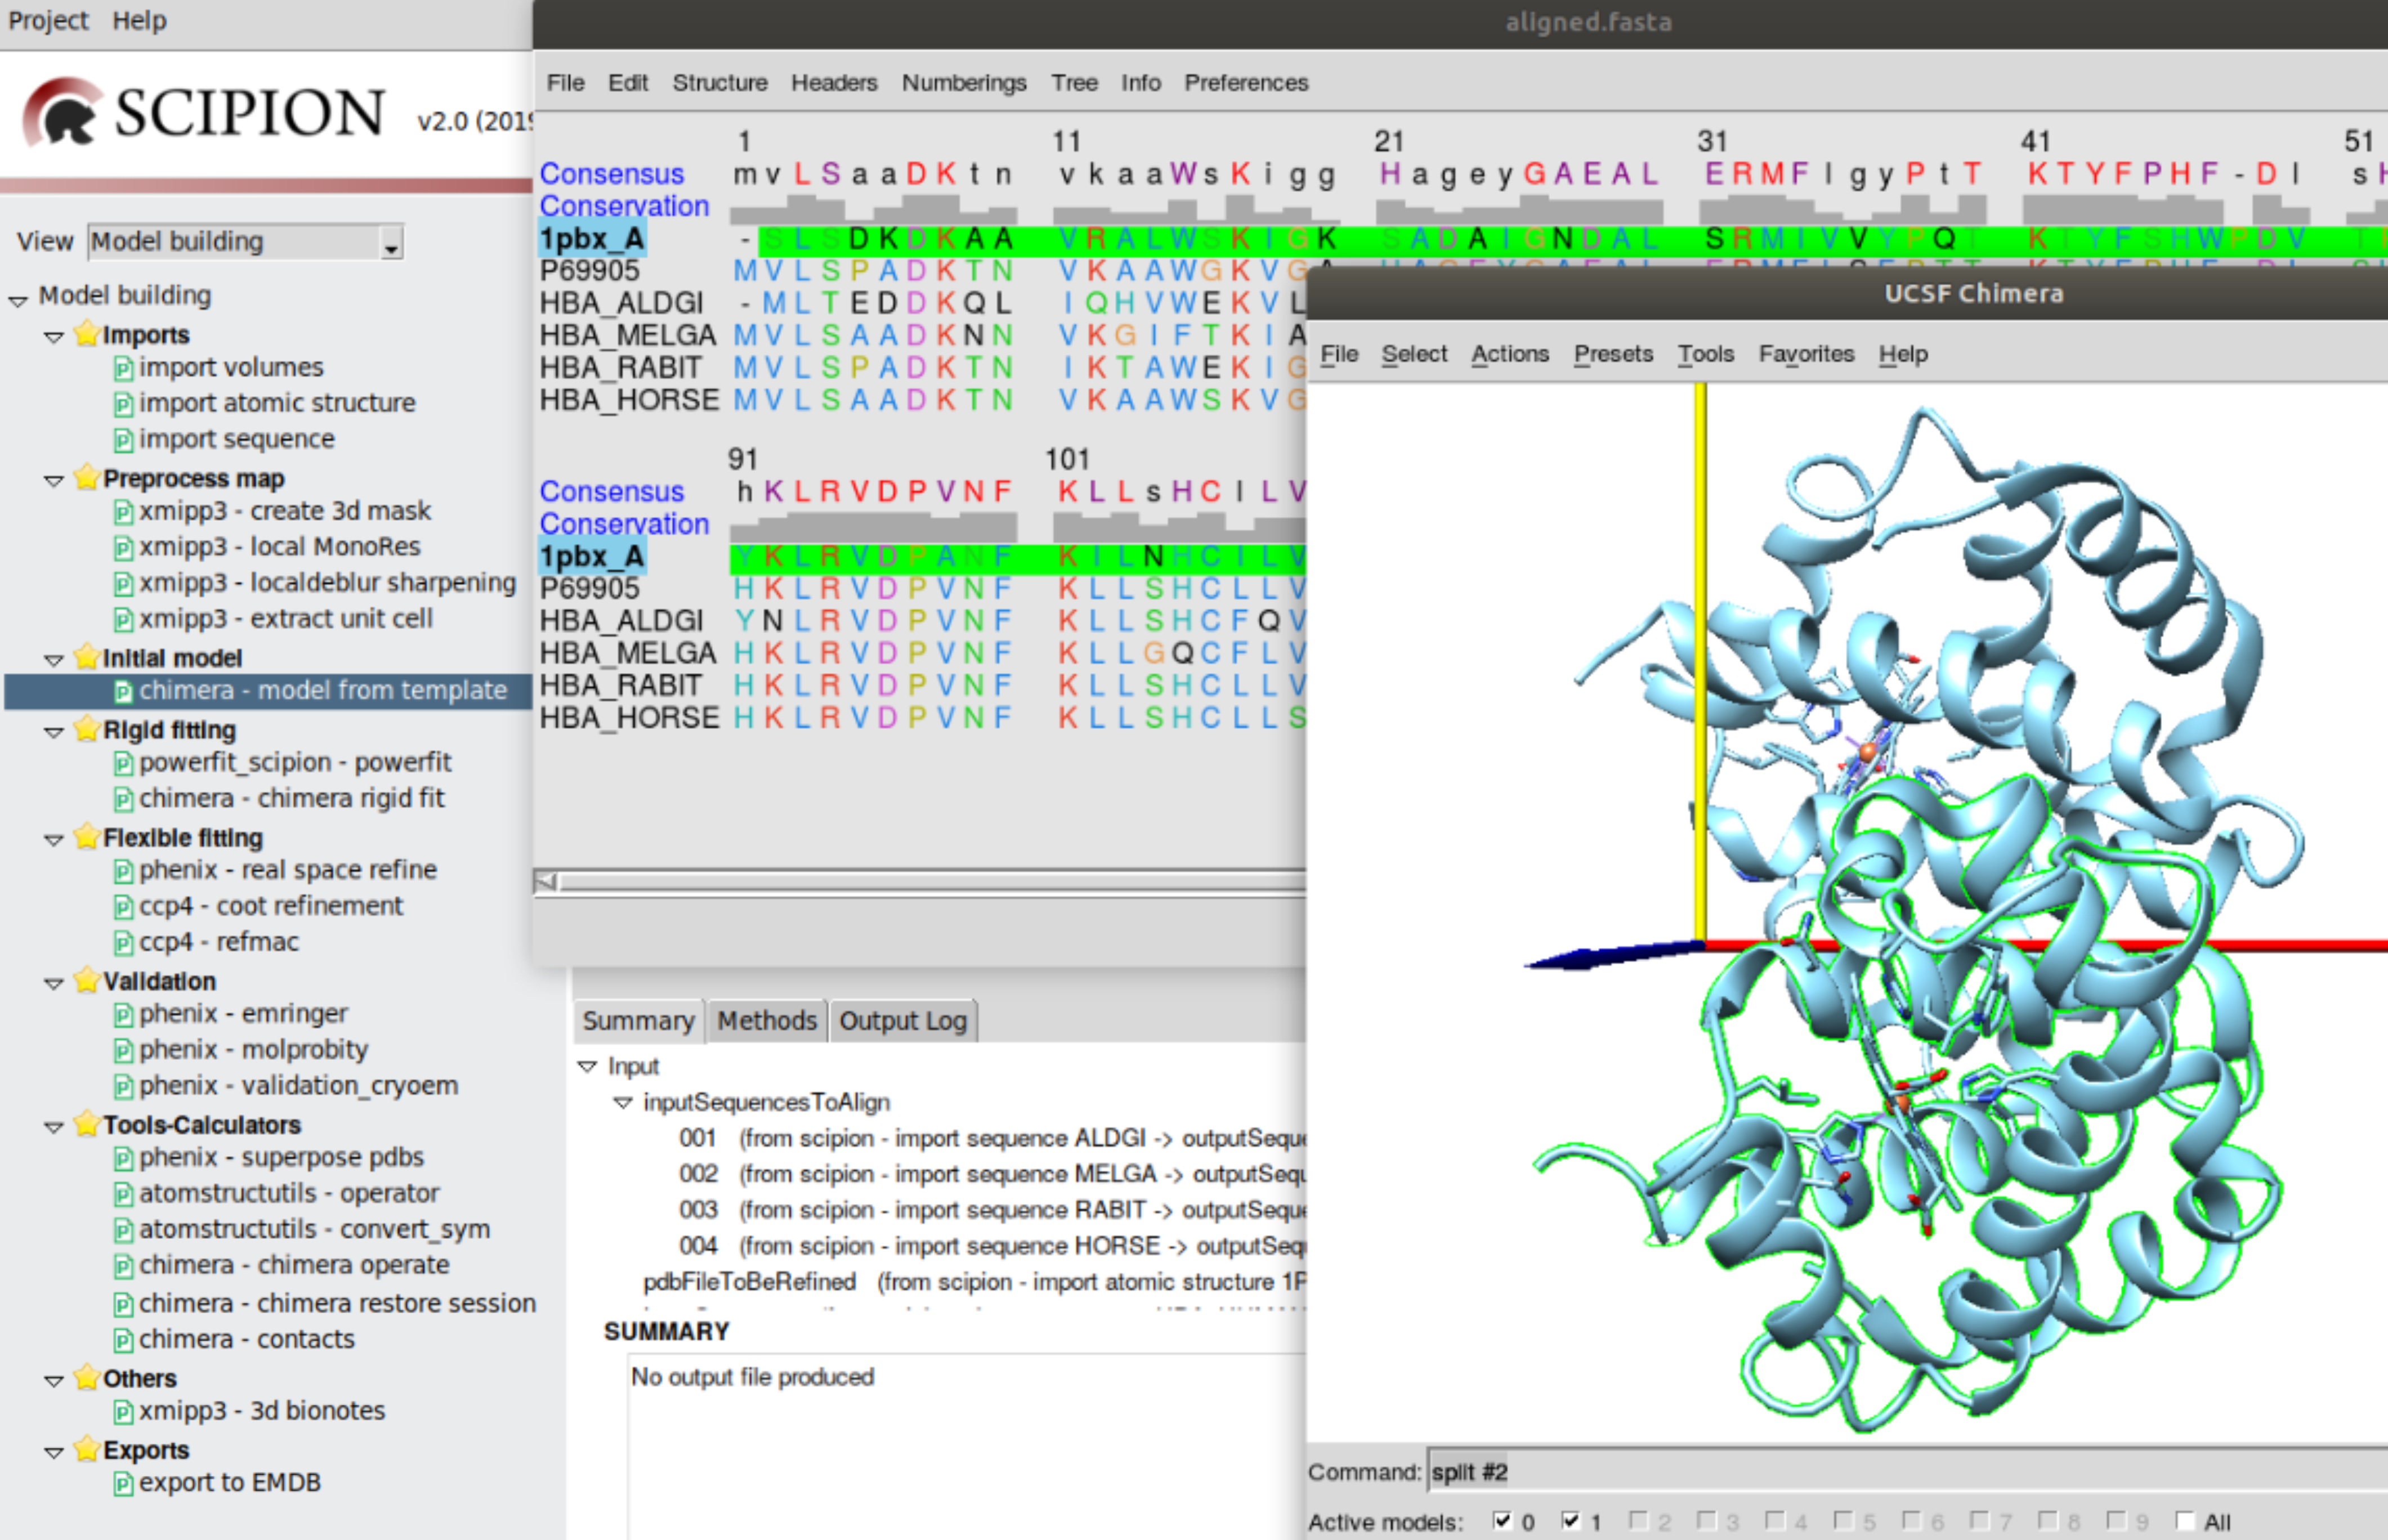
\includegraphics[width=0.80\textwidth]{Images/Fig14}
  \caption{Opening the multiple sequence alignment in \chimera.}
  \label{fig:chimera_alignment}
  \end{figure}
\end{itemize}

In case you'd like edit the name or the order of the sequences, add,  delete or realign sequences, ..., go to the upper menu of the multiple sequence alignment (\ttt{Edit -> }). In particular, we are going to change the name of the \iii{target} sequence from \ttt{P69905} to \ttt{HBA\_HUMAN} in \ttt{Edit -> Edit Sequence Name...} (\ffigure{fig:modeller} (A)). To get possible atomic models of the \iii{target} sequence in \modeller web service, we have to select \ttt{Structure -> Modeller (homology ...)} in the same upper menu. A new window for Comparative Modeling with Modeller will be open (\ffigure{fig:modeller} (B)), that we have to fill in selecting \iii{target} sequence (1) and \iii{template} (2). Modeller license key has to be included here (3). The number of output models can be specified in Advanced Options (5 by default). Finally, press Apply to start the computation without hide the panel (4) or OK to start the computation hiding it. In \chimera main graphics window, lower left corner, you may see the status of your job. After a while, five possible atomic structures, from now ahead \iii{models}, are retrieved for the \iii{target} sequence (\ffigure{fig:modeller} (C)) together with their assessment scores. Column \ttt{GA341} of Modeller Results indicates the score derived from statistical potentials (values in \ttt{[0,1]}; \ttt{> 0.7} for reliable \iii{models}). Column \ttt{zDOPE} (normalized Discrete Optimized Protein Energy) score depends on the atomic distance (negative values for the better \iii{models}). Let's select \iii{model} \ttt{\#2.1}. You can check every model numbers in \chimera's main menu (\ttt{Favorites -> Model Panel}).
 
  \begin{figure}[H]
  \centering 
  \captionsetup{width=.7\linewidth} 
  \includegraphics[width=0.80\textwidth]{Images/Fig15}
  \caption{(A) Sequence edition. (B) Completing the form to access to homology modeling with \modeller. (C) Resulting \iii{models}.}
  \label{fig:modeller}
  \end{figure}
 
 Comparing your selected \iii{model} of human \ttt{metHgb} $\alpha$ subunit with \ttt{1PBX\_A} \iii{template}, we observe that the selected \iii{model} \ttt{\#2.1} does not contain the \ttt{HEME} prosthetic group (\ffigure{fig:chimera_model} (A)). Before saving the \iii{model}, the \iii{template} \ttt{HEME} group will thus be added to your \iii{model} in \chimera. With this aim, open \chimera's command line; from \chimera main menu (\ttt{Favorites -> Command Line}) and delete every atom of \ttt{1PBX} \iii{template}, except the \ttt{HEME} group associated to chain \ttt{A}. To preserve residue 144 (\ttt{HEME} group) in chain \ttt{A}, write the next command line (\ffigure{fig:chimera_model} (A)(1)):
 \begin{verbatim}
     delete #1:0-143.A, 145-.A, .B
 or
     delete #1:0-143.A
     delete #1:145-.A
     delete #1:.B
 \end{verbatim}
 
 Go to the Model Panel and select models \ttt{\#1} and \ttt{\#2.1} simultaneously, then press \ttt{Copy/Combine} on the right side column (\ffigure{fig:chimera_model} (B)(2)). Model Panel shows the new \iii{model} created \ttt{\#3} (3), that we can save in the command line (4) writing:\\
 
 \ttt{scipionwrite model \#3}\\
 
 \begin{figure}[H]
  \centering 
  \captionsetup{width=.7\linewidth} 
  \includegraphics[width=0.80\textwidth]{Images/Fig16}
  \caption{\iii{Model} selection in \chimera. (A) Selected \iii{model} \ttt{\#2.1}. (B) Creation of full final \iii{model} of human \ttt{metHgb} $\alpha$ subunit, including \ttt{HEME} group.}
  \label{fig:chimera_model}
  \end{figure}
 
 After closing \chimera, you can visualize (\ffigure{fig:model_from_template_protocol} (8)) your full predicted \iii{model}. In a similar process, you can also obtain human \ttt{metHgb} $\beta$ subunit. %Remark that in this case, the \ttt{HEME} group will be kept with the next \chimera command line: \\
 %\ttt{delete \#1:.A, 0-147.B, 149-.B}\\ or \\
 %\ttt{delete \#1:.A}\\ \ttt{delete \#1:0-147.B}\\ \ttt{delete \#1:149-.B}\\
 Use this time a direct way of keeping the \ttt{HEME} group in your $model$ of \ttt{metHgb} $\beta$ subunit: Select the advanced option \ttt{Include non-water HETATM residues from template} included in  \ttt{Comparative Modeling with Modeller} window (\ffigure{fig:modeller} (B)).\\
  
If for any reason you decide to go back and check a different \iii{model} from the five \iii{models} initially provided by \modeller, you can do it by using \scommand{chimera restore session} protocol (Appendix \ref{app:chimeraRestoreSession}). This protocol may be used whenever \chimera session had been saved, specifically after using protocols \chimera \ttt{rigid fit}, \chimera \ttt{operate}, and \chimera \ttt{model from template}. In addition to the \chimera command line \ttt{scipionss}, command line \ttt{scipionwrite} also saves \chimera session by default. So, if you want to restore a previous session just open the form (\ffigure{fig:restore_session_protocol}, 1), and include the session that you'd like to restore (2).

 \begin{figure}[H]
  \centering 
  \captionsetup{width=.7\linewidth} 
  \includegraphics[width=0.90\textwidth]{Images/Fig17}
  \caption{Restoring session in \chimera.}
  \label{fig:restore_session_protocol}
  \end{figure}

\section{Volume and models scenario: Rigid Fitting}
Once we have the predicted \ttt{model} of any structural element included in our map, fitting that \ttt{model} in the volume constitutes the next step in the modeling workflow. Two protocols have been included in \scipion with this purpose, \scommand{powerfit} (Appendix \ref{app:powerfitProtocol}, \citep{vanzundert2016}) and \scommand{chimera rigid fit} (Appendix \ref{app:chimeraRigidFit}). The first one allows automatic fitting of models in maps, while the second only does it when model and map are quite close, thus requiring manual fitting in advance. Although there is no a general rule to fit map and model, because it will depend on the particular problem and on our previous knowledge, in this tutorial we are going to use $PowerFit$ application first, followed by the final \ttt{Fit in Map} in $Chimera$ \ttt{rigid fit}.

\begin{itemize}
 \item Initial rigid fit with $PowerFit$:\\
 Open \scommand{powerfit} protocol ((\ffigure{fig:powerfit_protocol} (1)), and complete the form with the full \iii{model} of atomic structure previously saved in $Chimera$ (2), the extracted unit cell volume (3), and volume resolution (4). Among the advanced parameters, consider carefully the angular step (5) according to the size of your volume and your computing power. Despite getting a more accurate result, fitting of big volumes takes more time as  lower values of angular step are given.  
 
 \begin{figure}[H]
  \centering 
  \captionsetup{width=.7\linewidth} 
  \includegraphics[width=0.85\textwidth]{Images/Fig18}
  \caption{Rigid fit with $PowerFit$: Filling in the protocol form.}
  \label{fig:powerfit_protocol}
  \end{figure}
 
 After executing the \scommand{powerfit} protocol, you can check results ((\ffigure{fig:powerfit_results_table} (A)(1)). The first table opened allows you to check the fitting quality (2) of best score-ordered fits in a second table (B). In our example only two fits are proposed. You can check which one fits better to the map by writing the selected fit number in the \ttt{Model to visualize} square window, and then displaying the fitting (3).
 
 \begin{figure}[H]
  \centering 
  \captionsetup{width=.7\linewidth} 
  \includegraphics[width=0.85\textwidth]{Images/Fig19}
  \caption{Rigid fit with $PowerFit$: Checking results by score.}
  \label{fig:powerfit_results_table}
  \end{figure}
  
  \ffigure{fig:powerfit_results_figs} shows the fitting of the two possible fits between map and \ttt{models} posed by $PowerFit$ (\ttt{fit\_1.pdb}, A, and \ttt{fit\_2.pdb}, B, green- and pink-colored, respectively). Although both of them seem to fit quite well the extracted unit cell map, only one of them should be OK. The other $model$ one must misfit the volume area that corresponds to \ttt{metHgb} $\beta$ subunit. This anomalous behavior of our \iii{model} is not surprising because \ttt{Hgb} $\alpha$ an $\beta$ subunits are 42.86\% sequence identical. 
  
 \begin{figure}[H]
  \centering 
  \captionsetup{width=.7\linewidth} 
  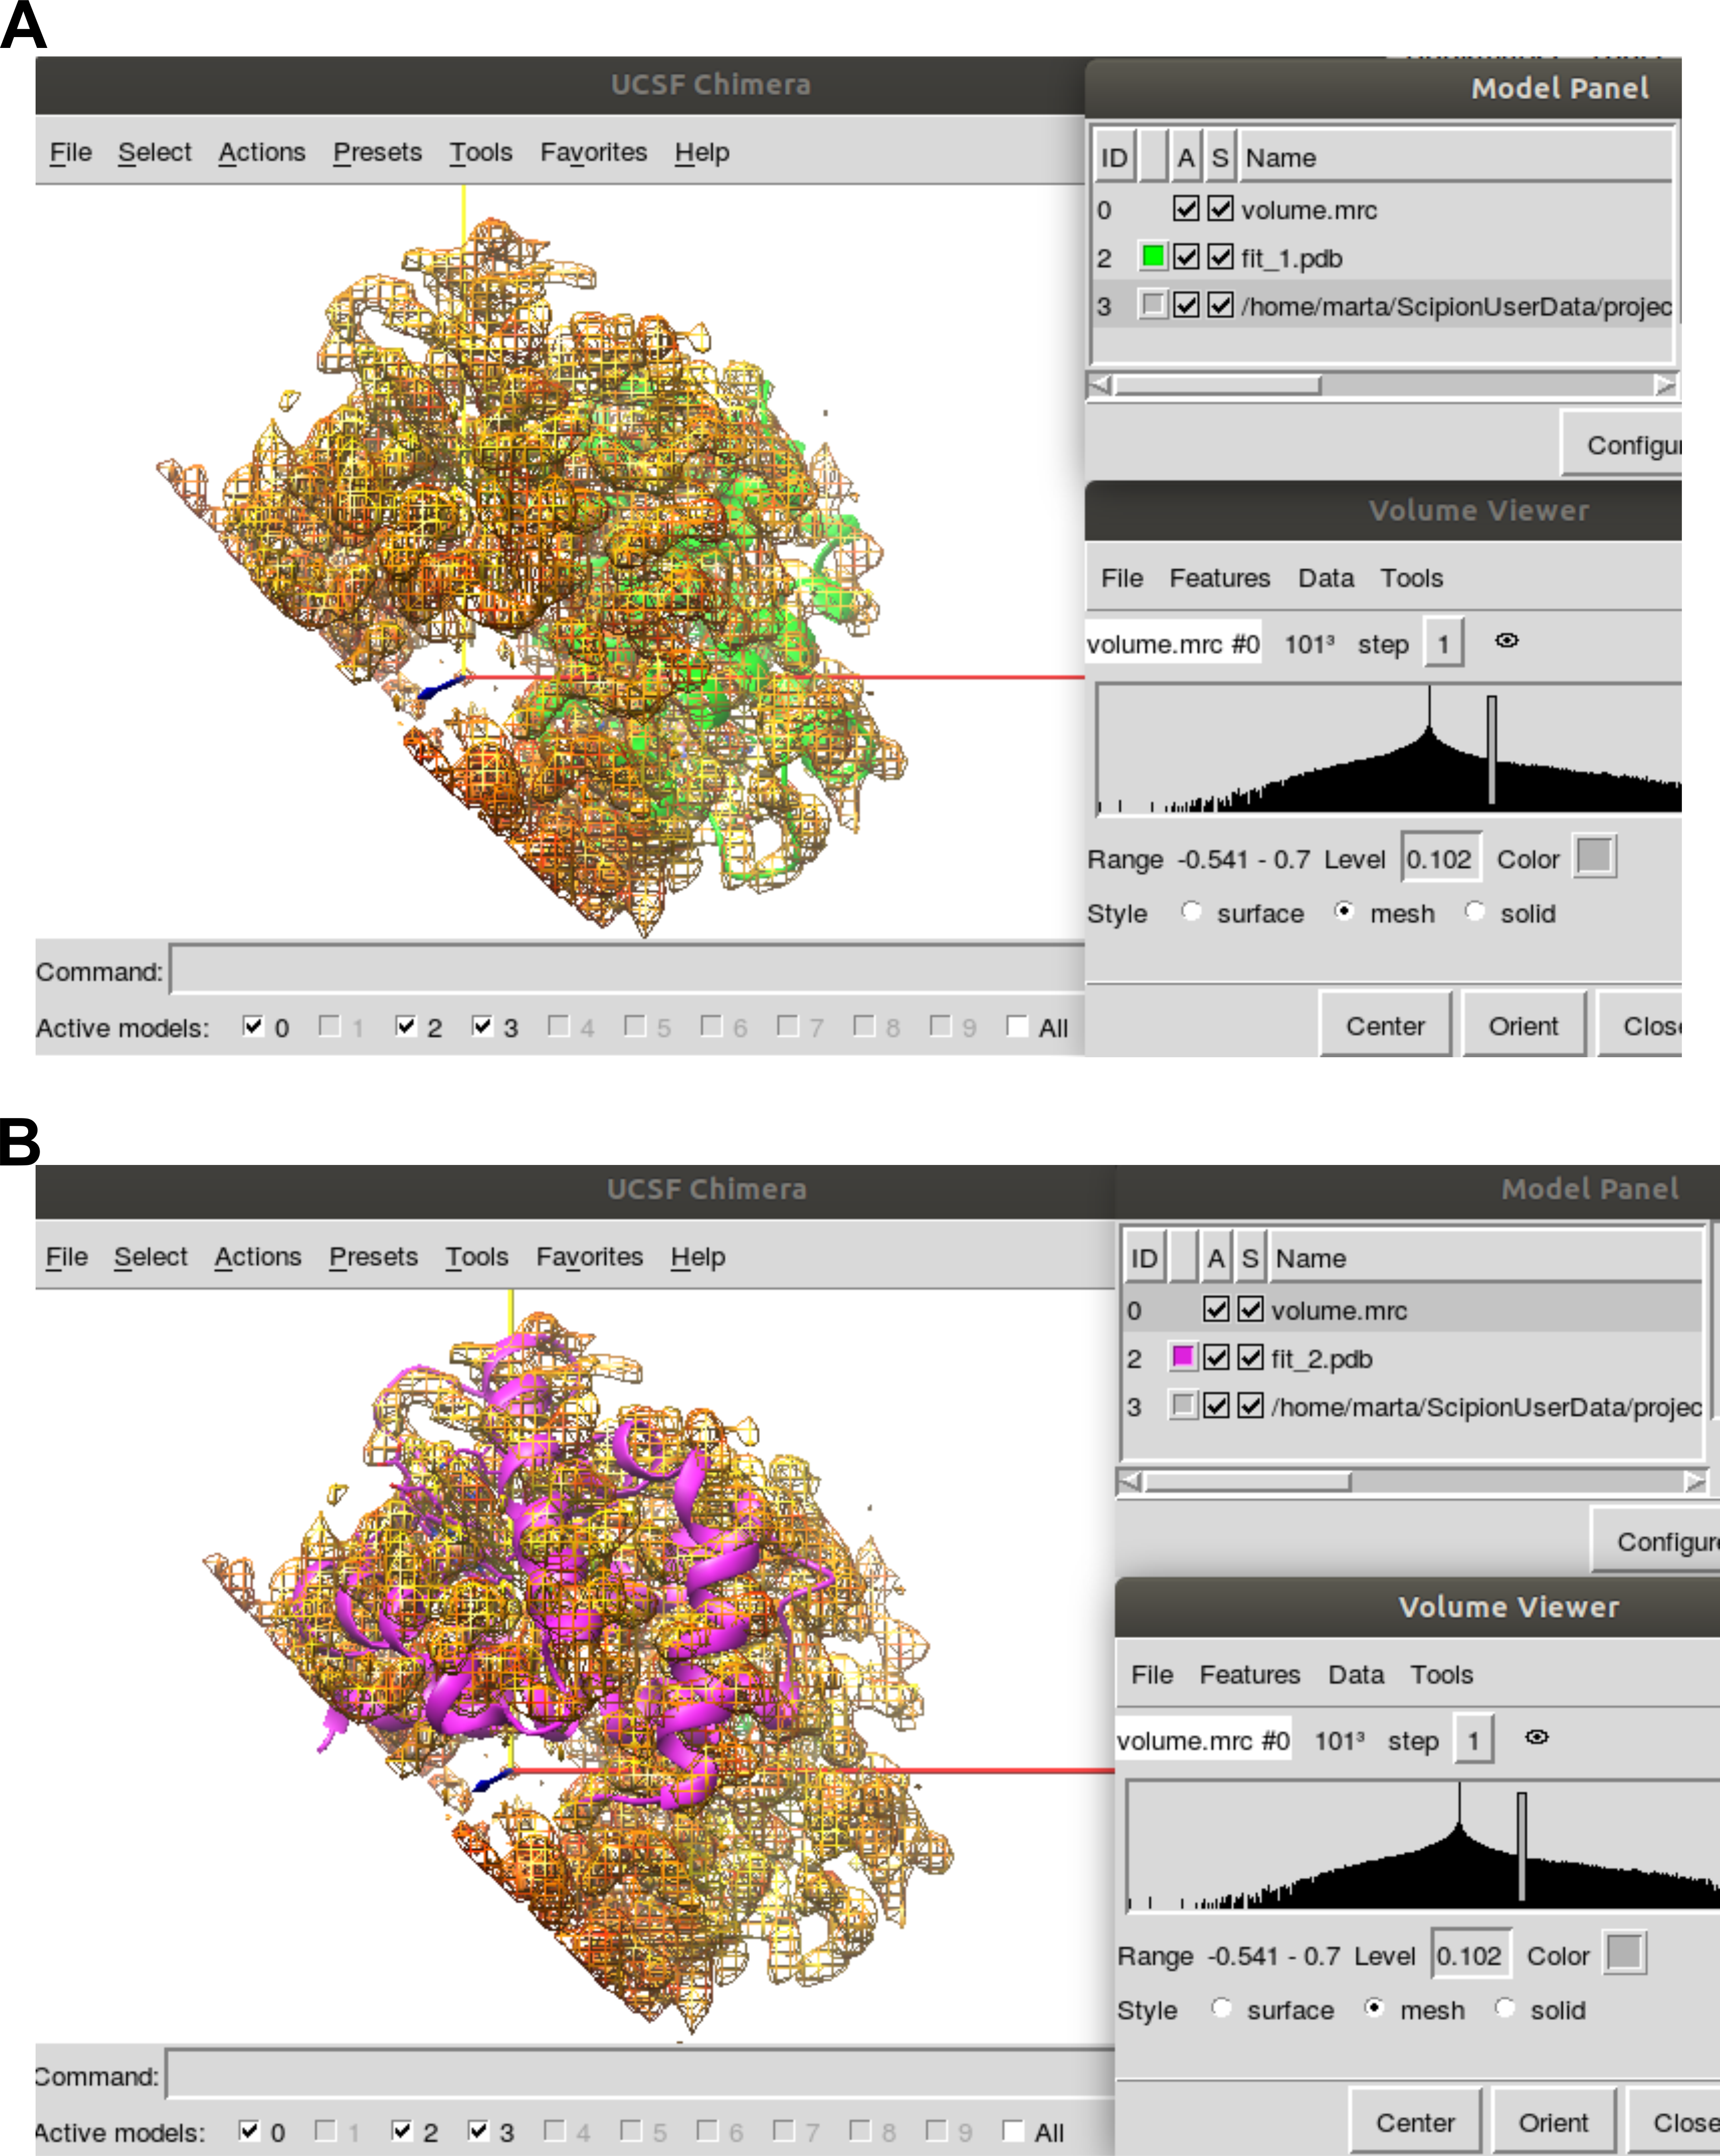
\includegraphics[width=0.85\textwidth]{Images/Fig20}
  \caption{Rigid fit with $PowerFit$: Checking the best fits in $Chimera$.}
  \label{fig:powerfit_results_figs}
  \end{figure}
  
 \item Completing rigid fit with $Chimera$ \ttt{rigid fit}:\\
 In order to assess which one of the structures fits the map better, the fitting has to be improved with \scommand{chimera rigid fit} protocol. Open this protocol (\ffigure{fig:chimera_rigid_fit} (1)), include the extracted unit cell as volume (2), one of the structures fitted (3), the other one (4), and execute the protocol.
 
 \begin{figure}[H]
  \centering 
  \captionsetup{width=.7\linewidth} 
  \includegraphics[width=0.85\textwidth]{Images/Fig21}
  \caption{Completing the $Chimera$ rigid fit protocol form.}
  \label{fig:chimera_rigid_fit}
  \end{figure}
  
  Once opened $Chimera$ graphical window, select in the upper main menu \ttt{Tools -> Volume Data -> Fit in Map}. A small window will be opened. Select each one of the fits in \ttt{Fit} and press \ttt{Fit} to allow the automatic rigid fitting. At the lower right side of \ffigure{fig:chimera_fit_in_map}, respective windows of \ttt{Fit in map} for \ttt{fit\_1.pdb} and \ttt{fit\_2.pdb} are detailed. In spite that the amount of \ttt{atoms outside the contour} is higher in \ttt{fit\_1.pdb} than in \ttt{fit\_2.pdb}, we can not conclude that the second fitting is better than the first one, because the \ttt{Average map value} is also lower. Visual inspection of both fits should identify the appropriate fitting of \iii{model} in map.
  
  \begin{figure}[H]
  \centering 
  \captionsetup{width=.7\linewidth} 
  \includegraphics[width=0.85\textwidth]{Images/Fig22}
  \caption{Fitting in map with $Chimera$.}
  \label{fig:chimera_fit_in_map}
  \end{figure}
  
  Suggestion before starting the visual inspection in $Chimera$: Check first the parts of the structure that could differ the most between \ttt{metHgb} $\alpha$ and $\beta$ subunits. These parts that differ the most can be identified by performing an additional alignment including the $\beta$ subunit sequence. \ffigure{fig:multiple_alignment_HBB} incorporates the $\beta$ subunit sequence (in yellow) to the alignment shown in \ffigure{fig:chimera_alignment}. Two regions that contain gaps of sequence are remarked in red frames. The first one, involving residues 19 and 20, absent in $\beta$ subunit, and the second one, after residue 51, could be the most relevant to differentiate between subunits. Look at them and identify the correct fit. You can highlight those residues in $Chimera$ writing in the command line:\\
  \ttt{sel :19-20}\\
  \ttt{sel :50-55}
  
  \begin{figure}[H]
  \centering 
  \captionsetup{width=.7\linewidth} 
  \includegraphics[width=0.85\textwidth]{Images/Fig23}
  \caption{Multiple sequence alignment including \ttt{Hgb} $\beta$ subunit (\ttt{HBB\_HUMAN}).}
  \label{fig:multiple_alignment_HBB}
  \end{figure}
  
  Once identified the appropriate fit, you can save it as fitted $model$ of the \ttt{metHgb} $\alpha$ subunit. Replacing \ttt{n} by your $model$ number (\ttt{1}, \ttt{2}), write in the command line of $Chimera$ graphical window:\\
  
  \ttt{scipionwrite model \#n refmodel \#1 saverefmodel 0}\\
  
In case you are still unable to decide which one is the best fit, don't worry. You will make your mind up with the next step in the workflow, but then save both fits with \ttt{scipionwrite} $Chimera$ command line. Don't forget to change the $model$ number. Your fitted models will be saved by $Chimera$ with names \ttt{chimeraOut0001.pdb} and \ttt{chimeraOut0002.pdb}.
 
\end{itemize}

\section{Refinement: Flexible fitting}
\label{refinementFlexibleFitting}
Although the rigid fitting approximates map and atomic $model$, a detailed visual inspection of map and model reveals that part of residues are not perfectly fitted. In order to get a better fit, not only of the carbon skeleton but also of residue side chains, a flexible fitting or refinement has to be accomplished. Refinement can thus be defined as the optimization process of fitting $model$ parameters to experimental data. Different strategies, categorized as refinement in the real space and refinement in Fourier space, can be followed. Implemented in \scipion are two protocols for real space refinement, \scommand{ccp4 - coot refinement} (Appendix \ref{app:ccp4CootRefinement}, \citep{emsley2010}) and \scommand{phenix - real space refine} (Appendix \ref{app:realSpaceRefineProtocol}, \citep{afonine2018a}, and one protocol to refine in reciprocal space, \scommand{ccp4 - refmac} (Appendix \ref{app:ccp4Refmac}, \citep{vagin2004}).

 \subsection*{CCP4 \coot Refinement}
 
 Initially devoted to atomic models obtained by X-ray crystallography methods, \coot (from Crystallopgraphic Object-Oriented Toolkit) is a 3D computer graphics tool that allows simultaneous display of map and fitted $model$ to accomplish mostly interactive modeling operations. Although this tutorial does not try to show every functionality of \coot, but indicate how to open, close and save partial and final \coot refined structures in \scipion, some of \coot basic relevant commands will be shown. Initially, we are going to refine our \iii{moldel} with \coot. First of all, open \scommand{ccp4 - coot refinement} protocol (\ffigure{fig:coot_refinement_protocol} (1)), load the extracted unit cell volume (2), with electron density normalized to 1, and the fitted structure $model$ (3). Load also the second fit (4) if you are not still sure about the correct fitted structure. Reading the protocol Help is recommended. After executing the protocol (5), \coot graphics window will appear to start working. 
 
 \begin{figure}[H]
  \centering 
  \captionsetup{width=.7\linewidth} 
  \includegraphics[width=0.85\textwidth]{Images/Fig24}
  \caption{Filling in \coot refinement protocol.}
  \label{fig:coot_refinement_protocol}
  \end{figure}
  

  To check the objects downloaded in \coot, go to the second bar of the main menu and select \ttt{Display Manager}. Map \ttt{(output\_volume.mrc)} (number \ttt{\#2}) and models \ttt{chimeraOut0001.pdb} and \ttt{chimeraOut0002.pdb} (numbers \ttt{\#1} and \ttt{\#0}, respectively) are displayed. To start, we are going to identify the faired fitted $model$ to the density map in order to delete in the \ttt{Display Manager} menu the other $model$, which is misfitted. Visual inspection would clarify this point, although direct observation of the \ttt{Density fit analysis} might be a shorter way. With this aim, go to the main menu of \coot graphical window and select \ttt{Validate -> Density fit analysis}. This density analysis is compared for the two possible fitted \iii{models} in \ffigure{fig:coot_density_fit_analysis}. As you can see, model \ttt{chimeraOut0001.pdb} shows that residues 19, 20 and 22, framed in \ffigure{fig:multiple_alignment_HBB}, do not fit to the density map, as expected from the misfit of the $\alpha$ subunit in the density of the $\beta$ subunit.
 
 \begin{figure}[H]
  \centering 
  \captionsetup{width=.7\linewidth} 
  \includegraphics[width=0.85\textwidth]{Images/Fig25}
  \caption{\coot comparison of \iii{model} fit in the map density.}
  \label{fig:coot_density_fit_analysis}
  \end{figure}
  
  Go again to \ttt{Display Manager} and delete the \iii{model} \ttt{chimeraOut0001.pdb} pressing \ttt{Delete Model}. From now ahead, the \iii{model} \ttt{chimeraOut0002.pdb} will be refined in the next steps of the modeling workflow.\\
  
  Before starting the refinement, IDs of chains should be fixed. Current IDs of chains are \ttt{Chain A} and \ttt{Chain} (see \ffigure{fig:coot_density_fit_analysis}), and will be changed to \ttt{Chain HEME} and \ttt{Chain A}, respectively. This can be carried out going to main \coot menu and selecting \ttt{Edit -> Change Chain IDs}. Verify the identity of your \iii{model} molecule (\ffigure{fig:coot_change_name_ID} (1), select the initial Chain ID (2, 4), and write the new Chain ID (3, 5). Finally, press \ttt{Apply New Chain ID}.
 
 \begin{figure}[H]
  \centering 
  \captionsetup{width=.7\linewidth} 
  \includegraphics[width=0.85\textwidth]{Images/Fig26}
  \caption{\coot change chain ID of \iii{model} \ttt{chimeraOut0002.pdb}.}
  \label{fig:coot_change_name_ID}
  \end{figure}
  
  According to \ffigure{fig:coot_density_fit_analysis}, \ttt{MET} residue of the new chain \ttt{A} does not fit to the map density. Maybe this residue has been processed post-translationally, as we have anticipated in \textbf{Starting Input data} section. To solve this question, go to \coot main menu and select \ttt{Draw -> Go To Atom... -> Chain A -> A 1 MET} (\ffigure{fig:coot_go_to_atom} (A)). \ttt{MET} residue will be located in the center of \coot graphics window. Check if this residue is surrounded by any electron density. As \ffigure{fig:coot_go_to_atom} (B)(1) shows, no density associates to the first chain residue. \ttt{MET} will thus be deleted. Then go to the lower right side menu and select the symbol to delete items (B)(2). Select \ttt{Residue/Monomer} in the opened \ttt{Delete item} window, and click the \ttt{MET} residue that you want to delete. Go again to \ttt{Validate -> Density fit analysis} and check that the red bar shown in \ttt{MET} residue (\ffigure{fig:coot_density_fit_analysis}) has disappeared.
  
  \begin{figure}[H]
  \centering 
  \captionsetup{width=.7\linewidth} 
  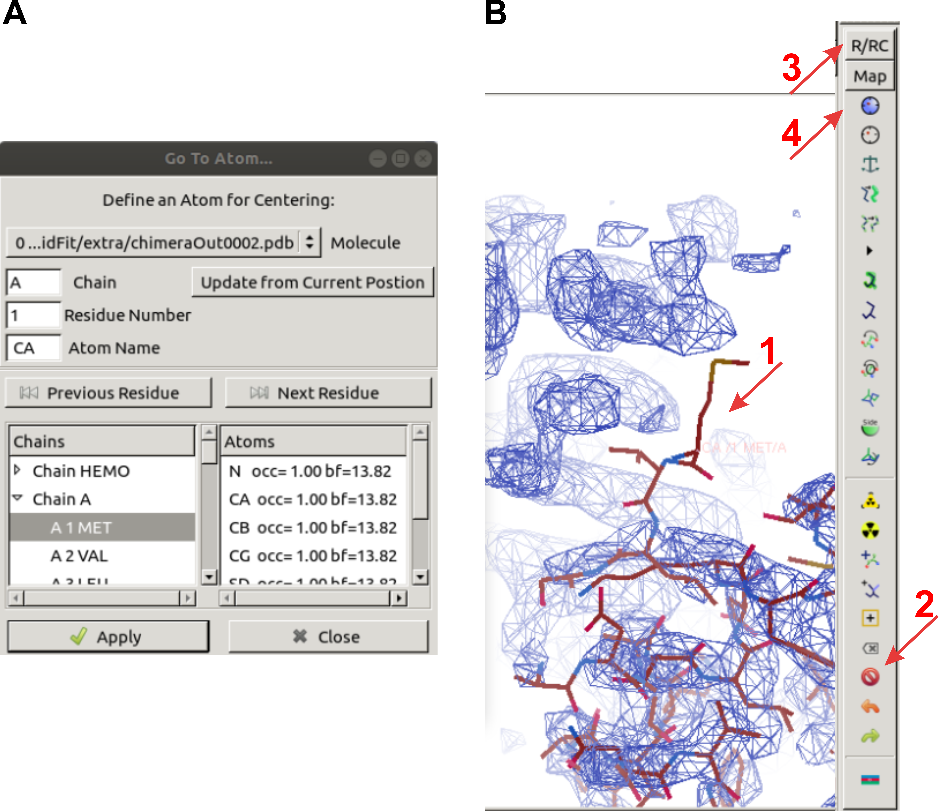
\includegraphics[width=0.80\textwidth]{Images/Fig27}
  \caption{Removing post-translationally processed Methionine residue in \coot. Note that the icons shown in the image right side may be partially hidden if the screen is small.}
  \label{fig:coot_go_to_atom}
  \end{figure}
  
  Before a more detailed visual inspection of the \iii{model} fitting, an initial quick refinement may be accomplished. With this purpose, first of all, go to the upper right side menu (\ffigure{fig:coot_go_to_atom} (B)(3)) and select all four restrictions for \ttt{Regularization and Refinement} in the respective window of parameters. Secondly, open the \ttt{coot.ini} text file, 
  open \scipion browser and navigate to the \ttt{extra} directory. Modify the file so it matches the information shown below (See \ffigure{fig:cootini}).\\
  \ttt{[myvars]}\\
  \ttt{imol: 0}\\
  \ttt{aa\_main\_chain: A}\\
  \ttt{aa\_auxiliary\_chain: AA}\\
  \ttt{aaNumber: 4}\\
  \ttt{step: 10}\\
  
  \begin{figure}[H]
  \centering 
  \captionsetup{width=.7\linewidth} 
  \includegraphics[width=0.80\textwidth]{Images/cootini}
  \caption{Edit coot.ini file.}
  \label{fig:cootini}
  \end{figure}
  
 %[**ROB coot need a careful presentation]
 %[**ROB preguntar a ERney por su metodo de filtracion]
 Finally, go back to \coot window and press ``U'' to initiate global variables and ``z'' to refine the next upstream 10 residues. Go through those residues, one by one, and accept refinement if you agree with it. If you disagree with the refinement of any residue, perform the interactive refinement, visualizing the residue side chain. Repeat the refinement process with ``z'' until the end of the molecule. Check that the orange bar of residue number 50 (\ffigure{fig:coot_density_fit_analysis}) goes missing at the end of this process.\\
 
 After this partially automatic and partially interactive processing, go to \ttt{Draw -> Go To Atom... -> Chain A -> A 2 VAL} (\ttt{VAL} is now the first residue of the \ttt{metHgb} $\alpha$ subunit) and start the detailed interactive refinement of the initial residues of chain A. To accomplish this interactive refinement of a small group of 5 to 10 residues, select the blue circle in the upper right side menu and click the initial and final residues of the small group of residues (\ffigure{fig:coot_go_to_atom} (B)(4)). The group of selected residues gets flexible enough to look manually for another spatial distribution. Following these instructions, try to solve the misfit that you can find in \ttt{TYR} 141 residue at the end of the molecule. Specifically, try to improve the result of the \ttt{Validate -> Density fit analysis}, as you can see from (A) to (B) in \ffigure{fig:coot_density_fit_analysis2}, moving \ttt{TYR} 141 ((A)(1)) to the nearest empty map density ((A)(2)). Accept the refinement parameters after the displacement of \ttt{TYR} ((B)(3)). Finally, check the \ttt{Density Fit Graph}.
 
  \begin{figure}[H]
  \centering 
  \captionsetup{width=.7\linewidth} 
  \includegraphics[width=0.85\textwidth]{Images/Fig28}
  \caption{\coot fit in the map density of residue \ttt{TYR} 141.}
  \label{fig:coot_density_fit_analysis2}
  \end{figure}
  
 Rotamer refinement is another refinement tool available in \coot. You can try to improve your current $model$ modifying rotamers reported as incorrect in \ttt{Validate -> Rotamer analysis}. Otherwise, the next refinement program in modeling workflow (\phenix \ttt{real space refine}) will perform rotamer refinement.\\
 
 At the end of this interactive refinement with \coot, the refined atomic structure has to be saved. You can save the atomic structure with its default name by pressing \keys{w}. If you prefer another name, for instance ``HBA\_HUMAN.pdb'', it can be saved in \coot main menu \ttt{Calculate -> Scripting -> Python} and the \ttt{Coot Python Scripting} window will be opened. Assuming that \ttt{0} is your \iii{model} number, write in Command:\\
 \ttt{scipion\_write (0, 'HBA\_HUMAN')}\keys{\return}
 
 In its interactive way, \scommand{ccp4 - coot refinement} protocol can be launched again whenever you want in \scipion, and the last atomic structure saved will be loaded in \coot graphics window. This functionality of \scipion allows to stop the interactive refinement and restart the process in the last refinement step, maintaining each one of the intermediate refined structures saved in order in \scipion tutorial folder \ttt{/Runs/000XXX\_CootRefine/extra}. In this way, go again to intermediate refined structures is also possible. Finally, when you reach the final refined structure save it, and you may press \keys{e} to fully stop protocol \coot.\\
 
 A similar refinement process to that followed in \coot for \ttt{metHgb} $\alpha$ subunit chain \ttt{A}, has to be carried out for chain \ttt{HEME} and for respective chains of \ttt{metHgb} $\beta$ subunit.\\
 
 
 \subsection*{\phenix Real Space Refine}
 
 In order to compare the previous \coot interactive refinement with an automatic refinement, we are going to use the
 \scommand{phenix - real space refine} protocol in parallel. This protocol implements in \scipion the \iii{phenix.real\_space\_refine} program developed to address cryo-EM structure-refinement requirements. Following a workflow similar to the \phenix reciprocal-space refinement program \iii{phenix.refine}, basically devoted to crystallography, \iii{phenix.real\_space\_refine} program, mainly used in cryo-EM, is able to refine in real space atomic models against maps, which are the experimental data.\\
 
 Start working by opening \scommand{phenix - real space refine} protocol (\ffigure{fig:phenix_real_space_refine_protocol} (1)), load as input volume the extracted unit cell saved in \coot (2), write the volume resolution (3), and load the atomic structure ($model$ \ttt{chimeraOut0002.pdb}, (4)). After executing the protocol (5), results can be checked (6). 
 
 \begin{figure}[H]
  \centering 
  \captionsetup{width=.7\linewidth} 
  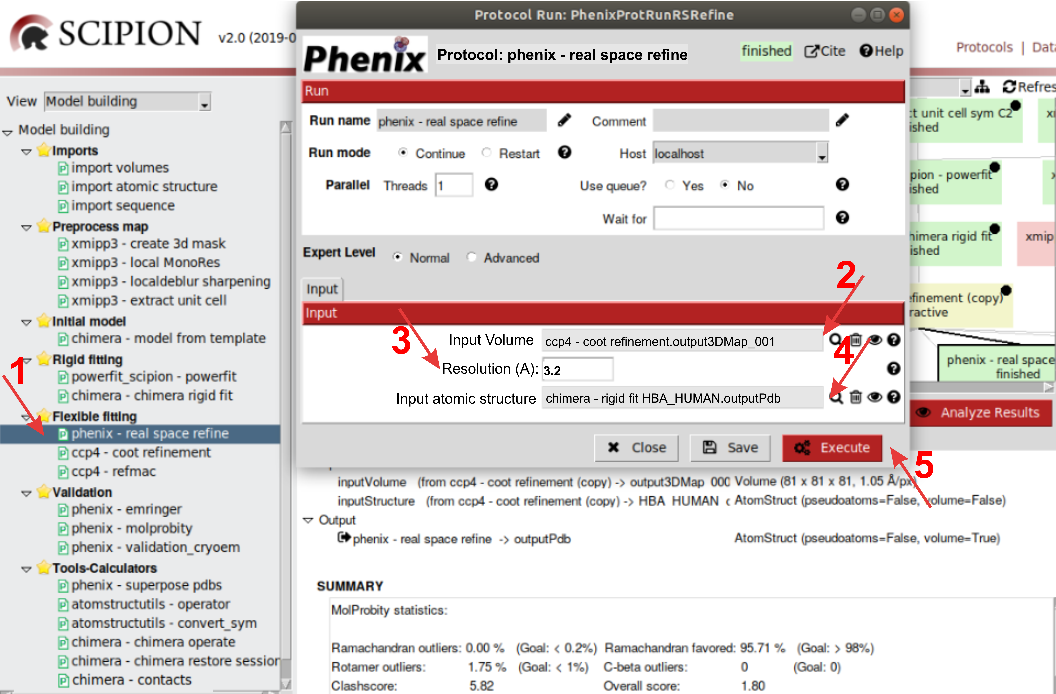
\includegraphics[width=0.85\textwidth]{Images/Fig29}
  \caption{Completing \phenix Real Space Refine protocol.}
  \label{fig:phenix_real_space_refine_protocol}
  \end{figure}
 
 The first tab of results shows the initial $model$ atomic structure as well as the refined one, both fitted to the normalized extract unit cell volume saved in \coot (\ffigure{fig:phenix_real_space_refine_chimera}). 
 
 \begin{figure}[H]
  \centering 
  \captionsetup{width=.7\linewidth} 
  \includegraphics[width=0.85\textwidth]{Images/Fig30}
  \caption{\chimera visualization of refined $model$ of \ttt{metHgb} $\alpha$ subunit by \phenix Real Space Refine protocol.}
  \label{fig:phenix_real_space_refine_chimera}
  \end{figure}
  
  The rest of tabs detail different statistics useful to compare the quality of distinct $models$ such as $MolProbity$ statistics and \ttt{Real-space} correlations. $MolProbity$ results will be discussed in the next section of validation and comparison. Regarding \ttt{Real-space} correlations, different $models$ can be compared by using the global number of \ccmask, that indicates the correlation $model$-to-map calculated considering the map region masked around the $model$. You can check also individual correlation values for each residue.  Remark that residues with lower correlation values might be susceptible to improve by additional refinement in \coot. Have a look to those correlation values and answer the following questions: (Answers in appendix \ref{app:solutions}; \textbf{Question \ref{refinementFlexibleFitting}\_1}) \\
  
  \begin{minipage}{\linewidth}
  \begin{framed}
  \begin{itemize}
  \item What is the \ccmask value?
  \item Which one is the residue that shows the lower correlation value? Why?
  \item What is that correlation value?
  \item Which one is the second residue that shows the lower correlation value? Why?
  \item What is that correlation value?
  \item What is the correlation value of \ttt{HEME} group?
  \end{itemize}
  \end{framed}
  \end{minipage}\\
  
  The conclusion of this part of refinement in real space is that \coot and \phenix \ttt{real space refine} might perform complementary tasks. The usage of both protocols may improve the result, especially when partial processing or big arrangements of molecules are involved. Now, to take advantage of $model$ improvements performed with \coot, run \phenix \ttt{real space refine} after \coot. When you finish, check again the above values of correlation. Have they changed? (Answer in appendix \ref{app:solutions}; \textbf{Question \ref{refinementFlexibleFitting}\_2})
  
  Before finishing our refinement workflow with \refmac, we can ask ourselves how can we improve correlations in real space by modifying the advanced parameters in the protocol form. Will the correlation values change if we set to ``yes'' optimization parameters previously set to ``no'', and increase the number of macro cycles from 5 to 30? Take into account that this process takes much more time (around 6 times more) than the previous one. (Answer in appendix \ref{app:solutions}; \textbf{Question \ref{refinementFlexibleFitting}\_3})\\
  
  \subsection*{\ccp4  \refmac}
  
  As in the case of \coot, \refmac (from maximum-likelihood Refinement of Macromolecules) was initially developed to optimize models obtained by X-ray crystallography methods but, unlike \coot, automatically and in reciprocal space. The $models$ refined in the real space with \coot and \phenix \ttt{real space refine}, successively, will be used as input to perform a second refinement step in the Fourier space with \refmac protocol \scommand{ccp4 - refmac}. Firstly, open the \refmac protocol form (\ffigure{fig:refmac_protocol} (1)), load the volume generated by \coot (2), the atomic structure obtained with \phenix \ttt{real space refine} (3), and the volume resolution as maximum resolution (4). Execute the protocol (5) and when it finishes, analyze the results (6).
  
  \begin{figure}[H]
  \centering 
  \captionsetup{width=.7\linewidth} 
  \includegraphics[width=0.85\textwidth]{Images/Fig31}
  \caption{Filling in \refmac protocol.}
  \label{fig:refmac_protocol}
  \end{figure}
  %[**ROB mask display in chimera is not centered **]
  Clicking the first item in the display menu of results (\ffigure{fig:refmac_display_results} (1)), \chimera graphics window will be opened showing the input volume, the initial $model$ (\ttt{HBA\_HUMAN} obtained with \phenix \ttt{real space refine}), and the final \refmac refined $model$ (\ffigure{fig:refmac_chimera}). By clicking the third item in the display menu of results (\ffigure{fig:refmac_display_results} (2)), a summary of \refmac results are shown. Check if values of \ttt{R factor} and \ttt{Rms BondLength} have improved with this refinement process. Why the improvement seems to be very small? (Answers in appendix \ref{app:solutions}; \textbf{Question \ref{refinementFlexibleFitting}\_4})\\
  
  Would you have seen a higher improvement running \refmac immediately after \coot, thus ignoring $model$ improvements generated by \phenix \ttt{real space refine}? (Answers in appendix \ref{app:solutions}; \textbf{Question \ref{refinementFlexibleFitting}\_5})\\
  
  Regarding the using of mask: Compare \refmac results (after \coot and \phenix \ttt{real space refine}) with those obtained selecting the option \ttt{No} in the protocol form parameter \ttt{Generate masked volume}. Use two different volumes, the one generated by \coot protocol, and the one generated by the \ttt{extract unit cell} protocol. Are there any differences? Why? (Answers in appendix \ref{app:solutions}; \textbf{Question \ref{refinementFlexibleFitting}\_6})\\
  
  \begin{figure}[H]
  \centering 
  \captionsetup{width=.7\linewidth} 
  \includegraphics[width=0.85\textwidth]{Images/Fig32}
  \caption{Display menu of \refmac results.}
  \label{fig:refmac_display_results}
  \end{figure}
  
  \begin{figure}[H]
  \centering 
  \captionsetup{width=.7\linewidth} 
  \includegraphics[width=0.85\textwidth]{Images/Fig33}
  \caption{\chimera visualization of refined $model$ of \ttt{metHgb} $\alpha$ subunit by \refmac.}
  \label{fig:refmac_chimera}
  \end{figure}
  
  Have a look to the rest of items in the display window of results. 
  

\section{Structure validation and comparison}

 At the end of the refinement process of \ttt{metHgb} $\alpha$ subunit (a similar one would be required for $\beta$ subunit), we need to assess the geometry of our $model$ regarding the starting 
volume to detect $model$ controversial elements or $model$ parameters that disagree with the map. Although each refinement program has their own tools to assess the progress of refinement ($Coot$ \ttt{Validate} menu; $Phenix$ \ttt{real space refine} real space correlations; $Refmac$ \ttt{R factor} and \ttt{Rms BondLength}), in this tutorial section, two assessment tools will be described to obtain comparative validation values after using any protocol in the workflow:  Protocols $EMRinger$ (\scommand{phenix - emringer}, Appendix \ref{app:emRingerProtocol}, \citep{barad2015}) and $MolProbity$ (\scommand{phenix - molprobity}, Appendix \ref{app:molprobityProtocol}, \citep{davis2004}). As in $Phenix$, correlation values in real space will be computed if a volume is provided with $MolProbity$ protocol. Additionally, we are going to introduce the protocol \scommand{phenix - superpose pdbs} (Appendix \ref{app:superposePdbsProtocol}, \citep{zwartUrl}) useful to compare visually the geometry of two atomic structures.\\

\begin{itemize}

 \item $EMRinger$:\\
 
 Specifically designed for cryo-EM data, $EMRinger$ tool assesses the appropriate fitting of a model to a map, validating high-resolution features such as side chain arrangements. The placement of side chains regarding the molecule skeleton depends on the $\chi_{1}$ dihedral angle, which is determined by atomic positions of \ttt{N}, \ttt{C$\alpha$}, \ttt{C$\beta$} and \ttt{C$\gamma$}. The $model$ backbone well fitted should be enriched in rotameric $\chi_{1}$ dihedral angles of 60º, 180º and 300º (-60º). The lower deviations regarding these values, the better $model$, and the higher EMRinger value.  
 
 We can start assessing with $EMRinger$ the \ttt{metHgb} $\alpha$ subunit $models$ that we have generated along the modeling workflow. In each case, open the \scommand{phenix - emringer} protocol ((\ffigure{fig:emringer_protocol} (1)), load the extracted unit cell volume (initial or saved with $Coot$) (2) and the atomic structure that you'd like to validate in relation to the volume (3), execute the program (4) and analyze results (5). A menu to check results in detail will be opened (bar \ttt{EMRinger results}). \iii{Phenix EMRinger} plots with density thresholds, with rolling window for each chain, as well as dihedral angles for each residue are shown here. The most relevant results, especially the EMRinger score, will also be written in the protocol \ttt{SUMMARY} (6). 
 
  \begin{figure}[H]
  \centering 
  \captionsetup{width=.7\linewidth} 
  \includegraphics[width=0.85\textwidth]{Images/Fig34}
  \caption{Completing $EMRinger$ protocol form.}
  \label{fig:emringer_protocol}
  \end{figure}
 
 Run $EMRinger$ protocol and determine the respective score after running \iii{PowerFit item2}, $Chimera$ \ttt{rigid fit} ($model$ 2), $Coot$ refinement, $Phenix$ \ttt{real space refine} after $Coot$ (default conditions and last modification of form parameters), and $Refmac$ refinement with MASK before and after $Phenix$ \ttt{real space refine}. Considering $EMRinger$ \ttt{score}, does our \ttt{metHgb} $\alpha$ subunit $models$ seem to be OK? (Answers in appendix \ref{app:solutions}; \textbf{Question 8}). Try the same validation with $\beta$ subunit $models$. \\
 
 \item $MolProbity$:\\
 
 The atomic structure validation web service $MolProbity$, with better reference data has been implemented in the open-source CCTBX portion of $Phenix$ \citep{williams2018}. This widely used tool assesses $model$ geometry and quality at both global and local levels. Originally designed to evaluate structures coming from X-Ray diffraction and NMR, it does not take into account the quality of the fitting with a 3D density map.  The implementation in $Phenix$, nevertheless, includes the possibility of adding a volume and assessing the correlation in the real space.\\
 
 The assessment process that we have carried out with $EMRinger$ can also be done with $MolProbity$ in \scipion. We are going to validate the geometry of \ttt{metHgb} $\alpha$ subunit $models$ that we have generated along the modeling workflow. In each case, open the \scommand{phenix - molprobity} protocol (\ffigure{fig:molprobity_protocol} (1)), load the extracted unit cell volume (initial or generated by $Coot$) (2) wit its resolution (3) if you want to have real space correlation between map and $model$, load the $model$ atomic structure (4) and execute the protocol (5). In \ttt{Analyze results} (6) the same menu bars available in results section of $Phenix$ \ttt{real space refine} protocol are shown here. $MolProbity$ results bar include validation statistics. Protocol \ttt{SUMMARY} emphasizes the most relevant ones.\\
 
 \begin{figure}[H]
  \centering 
  \captionsetup{width=.7\linewidth} 
  \includegraphics[width=0.85\textwidth]{Images/Fig35}
  \caption{Completing $MolProbity$ protocol form.}
  \label{fig:molprobity_protocol}
  \end{figure}
  
  Run $MolProbity$ protocol to obtain its statistics values after running \iii{PowerFit item2}, $Chimera$ \ttt{rigid fit} ($model$ 2), $Coot$ refinement, $Phenix$ \ttt{real space refine} (default conditions and last modification of form parameters) after $Coot$, and $Refmac$ refinement with MASK before and after $Phenix$ \ttt{real space refine}. In order to compare validation results of $models$ obtained along the modeling workflow, fill in the next table (\ttable{table:empty}) including, in addition to $MolProbity$ statistics, $EMRinger$ scores and \ccmask values obtained before. (Answers in appendix \ref{app:solutions}; \textbf{Question 9}). The same table (\ttable{table:empty}) can be completed for \ttt{metHgb} $\beta$ subunit (Appendix \ref{app:solutions}; \textbf{Question 10})\\
  
  \begin{sidewaystable}
   \caption{Validation statistics of human \ttt{metHgb} $\alpha$ subunit $model$. \ttt{RSRAC} stands for \ttt{Real Space Refine} after $Coot$. \ttt{Rama} stands for \ttt{Ramachandran}.}
   \centering\footnotesize
   \begin{tabular}{l c c c c c c c c}
   \hline\hline
   Statistic &  \thead{$Powerfit$\\ $item$ \#2} & \thead{$Chimera$\\ $model$ \#2} & $Coot$ & \thead{$Phenix$\\ \ttt{RSRAC}\\(default)} & \thead{$Phenix$\\ \ttt{RSRAC}\\(modified)} & \thead{$Refmac$\\ after $Coot$} & \thead{$Refmac$\\ after \ttt{RSRAC}\\(modified)} & \ttt{5NI1}\\ [0.5ex]
   \hline
   \ccmask \\
   $EMRinger$ \ttt{score} \\
   \ttt{RMS} (Bonds) \\
   \ttt{RMS} (Angles) \\
   \ttt{Rama favored} (\%) \\
   \ttt{Rama allowed} (\%) \\
   \ttt{Rama outliers} (\%) \\
   \ttt{Rotamer outliers} (\%) \\
   \ttt{Clashscore} \\
   \ttt{Overall score} \\
   \ttt{C$\beta$ deviations} \\
   \ttt{RMSD} \\[1ex] 
   \hline
   \end{tabular}
   \label{table:empty}
   \end{sidewaystable}
 
 
 Results compiled in this table indicate that statistics are uncorrelated. From the point of view of correlation in real space, the best $model$ was obtained from $Phenix$ \ttt{real space refine} (last modification of form parameters) after $Coot$. Considering $EMRinger$ \ttt{score}, the best $model$ derives from the whole workflow $Coot$ \ttt{->} $Phenix$ \ttt{real space refine} (default conditions). With $MolProbity$ \ttt{Overall score} as validation rule, the last step in the workflow could be suppressed because the best value was obtained after $Coot$ \ttt{->} $Phenix$ \ttt{real space refine} (last modification of parameters). We'd like to select the best $model$ and continue refining it in order to improve it as much as possible. Assuming that no one $model$ is perfect, how can we select the best one?\\ 


 \item $Model$ Comparison:\\
 
 The question posed in the previous item does not have an easy answer in the real world, in which we do not know the final atomic structure. In this tutorial, nevertheless, we know it and we can wonder how far we are of the atomic structure already published for this cryo-EM map. The question can be answered by comparing a) validation statistics that we have obtained for our $models$ with the statistics computed for the available $\alpha$ subunit in \ttt{PDB} structure \ttt{5NI1}, and b) the atomic structures themselves by overlapping.\\ 
    
  \begin{itemize}
  \item Comparison of validation statistics: \\
  
  Validation statistics of \ttt{metHgb} $\alpha$ subunit of \ttt{PDB} structure \ttt{5NI1} should be obtained as first step to compare them with our $models$ validation statistics. With this aim we are going to follow the next workflow:\\
  \begin{itemize}
    \item Protocol \scommand{import atomic structure}:\\
    Download from \ttt{PDB} structure \ttt{5NI1}\\
    
    \item Protocol \scommand{chimera operate} (Appendix \ref{app:chimeraOperate}):\\
    Similar to $Chimera$ \ttt{rigid fit}, $Chimera$ \ttt{operate} protocol allows to perform operations with atomic structures. We are going to use this protocol to save independently in \scipion the \ttt{metHgb} $\alpha$ subunit. Open the protocol  (\ffigure{fig:chimera_operate_protocol} (1)), complete the parameter \ttt{PDBx/mmCIF} including the atomic structure \ttt{5NI1} previously imported (2), and execute the protocol (3).      
    
    \begin{figure}[H]
    \centering 
    \captionsetup{width=.7\linewidth} 
    \includegraphics[width=0.90\textwidth]{Images/Fig36}
    \caption{Filling in $Chimera$ \ttt{operate} protocol form.}
    \label{fig:chimera_operate_protocol}
    \end{figure}
    
    The $Chimera$ graphics window will be opened with the structure \ttt{5NI1} as model number \#1. To save independently the structure of human \ttt{metHgb} $\alpha$ subunit (chain A), write in $Chimera$ command line:\\
    \ttt{split \#1}\\
    \ttt{scipionwrite model \#1.1}\\
    
    \item Protocol \scommand{powerfit}:\\
    Open $PowerFit$ protocol and follow the instructions above indicated. The structure saved in $Chimera$ operate will replace this time our previous $model$ (\ffigure{fig:powerfit_protocol} (2)). Select \ttt{item 2} as best fit.\\
    
    \item Protocol \scommand{chimera rigid fit}:\\
    Open again $Chimera$ \ttt{rigid fit} protocol and, following already indicated instructions, include this time \ttt{item 2}, the last fitted structure obtained with $PowerFit$ (\ffigure{fig:chimera_rigid_fit} (3)). After finishing the rigid fit of the extracted unit cell and \ttt{metHgb} $\alpha$ subunit from 5NI1 structure, you can save this fitted structure writing in $Chimera$ command line:\\
    \ttt{scipionwrite model \#2 refmodel \#1 saverefmodel 0}\\
    
    \item Validation protocols \scommand{phenix - emringer} and \scommand{phenix - molprobity}:\\
    Compute validation statistics with these two protocols for \ttt{metHgb} $\alpha$ subunit from \ttt{PDB} structure \ttt{5NI1}, write respective values in the previous table (\ttable{table:empty}), and compare them with the statistics of our $models$.
    
    Considering results shown in appendix \ref{app:solutions} (\textbf{Question 9}) for \ttt{metHgb} $\alpha$ subunit, we can conclude that published structures are not perfect and we are not very far from this published one. In fact, we have overcome every statistic except \ccmask. Then, the three different $models$ generated after $Coot$ refinement could be acceptable. \\

  \end{itemize}
 
  \item Comparison of atomic structures: \\
  
  $Phenix$ protocol \scommand{phenix - superpose pdbs} allows to compare two atomic structures by overlapping them. Root mean square deviation (RMSD) between the fixed structure (the published one) and one of our $models$ supports the classification of $models$ according to its proximity to the published model. Open $Phenix$ \ttt{superpose pdbs} protocol form (\ffigure{fig:superpose_pdbs_protocol} (1)), include the published structure of the \ttt{metHgb} $\alpha$ subunit as fixed structure (2), each one of the $models$ generated along the worflow (3) and execute the protocol (4). Finally, complete the \ttable{table:empty} with the value of RMSD obtained for each $model$. (Answers in appendix \ref{app:solutions}; \textbf{Question 9}).
  
  \begin{figure}[H]
    \centering 
    \captionsetup{width=.7\linewidth} 
    \includegraphics[width=0.90\textwidth]{Images/Fig37}
    \caption{Completing $Phenix$ \ttt{superpose pdbs} protocol form.}
    \label{fig:superpose_pdbs_protocol}
    \end{figure}
    
  You can check in $Chimera$ the fitted $model$ to the published structure by pressing \ttt{Analyze results} (\ffigure{fig:superpose_pdbs_protocol} (5)). Arrows of \ffigure{fig:superpose_pdbs_chimera} remark differing parts between both atomic structures. By opening these structures in $Coot$ you can see the difference between them.
 
   \begin{figure}[H]
    \centering 
    \captionsetup{width=.7\linewidth} 
    \includegraphics[width=0.90\textwidth]{Images/Fig38}
    \caption{$Model$ generated for \ttt{metHgb} $\alpha$ subunit superposed to published $\alpha$ chain of \ttt{5NI1} structure.}
    \label{fig:superpose_pdbs_chimera}
   \end{figure}
  
  
  \end{itemize}
 \end{itemize}
 
 A $model$ for \ttt{metHgb} $\alpha$ subunit has to be selected at the end of validation process. According to the statistics of \ttable{table:refmac_question_9} (Appendix \ref{app:solutions}; \textbf{Question 9}), $model$ obtained in the last step of modeling workflow ($Refmac$ after RSRAC (modified)) has been selected due to the smallest RMSD value, high value of $EMRinger$ \ttt{score}, quite high value of \ccmask and acceptable $MolProbity$ statistics. Follow a similar process to validate and select the $model$ generated for \ttt{metHgb} $\beta$ subunit. Appendix \ref{app:solutions} \textbf{Question 10} contains a statistics table for \ttt{metHgb} $\beta$ subunit, similar to that obtained for \ttt{metHgb} $\alpha$ subunit.\\
 
 In the real world, selected $models$ usually are the starting point to improve specific validation parameters by additional refinement. Since the improvement of certain parameters normally implies worsening of others, a final compromise solution has to be taken.\\



\section{Building the asymmetric unit}
\label{buildingunitcell}

Once we have selected the $models$ for \ttt{metHgb} $\alpha$ and $\beta$ subunits (see the workflow branches to have $\alpha$ and $\beta$ subunits \ffigure{fig:scipion_workflow_whole_reconstruction}), we can regenerate the smallest asymmetrical element of the starting map. With this aim we are going to use protocols to operate with atomic structures (\scommand{chimerax - operate} or \scommand{atomstructutils - operator}), to refine them both manually (\scommand{ccp4 - coot refinement}) and automatically (\scommand{phenix - real space refine}) and to validate them (\scommand{phenix - validation\_cryoem} and \scommand{phenix - emringer}). A brief schema of the main steps of this part of the workflow can be seen in \ffigure{fig:scipion_workflow_whole_reconstruction}. Take into account that in real live probably many more steps of refinement and validation will be required.\\ 

 \begin{figure}[H]
  \centering 
  \captionsetup{width=.9\linewidth} 
  \includegraphics[width=1\textwidth]{Images/Fig73}
  \caption{\scipion framework detailing the workflow to reconstruct the structure of the map asymmetric unit (blue arrow) and the whole atomic structure (red arrow).}
  \label{fig:scipion_workflow_whole_reconstruction}
  \end{figure}

\begin{itemize}
 \item Protocol to join the \ttt{metHgb} $\alpha$ and $\beta$ subunits in a unique atomic structure:\\ Two protocols can be used in \scipion for this purpose (\scommand{chimerax - operate} or \scommand{atomstructutils - operator}) and the result should be identical. \\
 Before starting, nevertheless, be sure that you have two atomic structures and each one includes an only chain with a different name. Remember that chain names should have changed for other chains than the first one before saving the refined atomic structure in \coot (\ffigure{fig:chimerax_asymm_unit_2}). Secondly, it could be very convenient to change the \scipion output label of each subunit, in order to follow them easily in \scipion. According to the \ffigure{fig:scipion_workflow_edition} go to the Summary of the two final protocols that allow to generate those atomic structures and press the black arrow (C) to select the option \ttt{Edit}. Type the new output name of the structures (\ttt{HBA\_refined} (D) and \ttt{HBB\_refined} (E), respectively).\\
    
  \begin{figure}[H]
  \centering 
  \captionsetup{width=.9\linewidth} 
  \includegraphics[width=1\textwidth]{Images/Fig75}
  \caption{A. Zoom in on \ffigure{fig:scipion_workflow_whole_reconstruction}. B. Summary of the protocol box from \phenix \ttt{real space refine} ($\alpha$ in (A)). Red arrow points at the \scipion output name. C. Menu opened pressing the output black arrow of the Summary. D. New name of the \scipion output in the Summary. E. Summary from the protocol box \phenix \ttt{real space refine} ($\beta$) after applying the same edition process.}
  \label{fig:scipion_workflow_edition}
  \end{figure}
  
  Then, open again $ChimeraX$ \ttt{operate} protocol and following the already indicated instructions, include the $models$ of \ttt{metHgb} $\alpha$ and $\beta$ subunits in params \ttt{Atomic structure} and \ttt{Other atomic structures}, respectively (\ffigure{fig:chimerax_asymm_unit_1} (A)). Firstly, check that both \ttt{models} are perfectly fitted in the map asymmetric unit. Otherwise, apply the command \ttt{fitmap}, as it was previously shown. Next, create a single atomic structure by joining models \ttt{\#3} and \ttt{\#4} in $ChimeraX$ \ttt{Models} panel. To generate a combined \ttt{model} write in the command line:\\
  \\ \ttt{scipioncombine \#3,4}\\
  \\The new model \ttt{\#5} is shown in $ChimeraX$ \ttt{Models} panel (\ffigure{fig:chimerax_asymm_unit_1}). Finally, save this fitted structure writing in $ChimeraX$ command line:\\ 
  \\ \ttt{scipionwrite \#5 prefix asymmetric\_unit\_model\_}\\ 
    
  \begin{figure}[H]
  \centering 
  \captionsetup{width=.9\linewidth} 
  \includegraphics[width=1\textwidth]{Images/Fig76}
  \caption{A. Completing the \scommand{chimerax - operate} protocol with the atomic structures \ttt{HBA\_refined} and \ttt{HBB\_refined} . B. \chimera graphics window showing the combined \ttt{model \#5}.}
  \label{fig:chimerax_asymm_unit_1}
  \end{figure}

 \item Protocols to refine the new combined structure generated:\\
  
At this point refinements could cover specially the overlapping area between the two chains. Help yourself with the \coot tools of \ttt{Validate} in the main menu, as well as the visualization tools of \phenix \ttt{real space refine} protocol. 
 \item Validation protocols to select the best $model$ of the human \ttt{metHgb} unit cell:\\
 \\Validate the new combined structure generated is recommendable before continuing with the next steps in the workflow.$EMRinger$ and $Validation CryoEM (MolProbity)$ validation statistics should be computed for the new $model$ of human \ttt{metHgb} asymmetric unit, generated by combining \ttt{metHgb} $\alpha$ and $\beta$ subunits. Appendix \ref{app:solutions} (\textbf{Question \ref{buildingunitcell}\_1}) contains a statistics table for the unit cell $model$ (\ttable{table:refmac_question_11}). We can try to improve those statistics by additional refinement processes. By performing refinement in real space with $Phenix$ some of the statistics could result improved. \ttable{table:refmac_question_11} contains also RMSD values computed in a similar way as we have seen for $\alpha$ and $\beta$ subunits, considering as fixed structure chains A and B from \ttt{5NI1} atomic structure. To continue with the modeling process we can select the unit cell $model$ generated by $Phenix$ \ttt{real space refine} because most of its validation statistics show the best values (\ccmask, $EMRinger$ \ttt{score} and $MolProbity$ values). Exceptionally, RMSD regarding the published structure yields the worst value.
 
\end{itemize}


\section{The whole macromolecule}
\label{wholemacromolecule}

To regenerate the whole human \ttt{metHgb} macromolecule, we are going to follow basically the schema shown in \ffigure{fig:scipion_workflow_whole_reconstruction}. Starting from the symmetric unit, \chimera \ttt{operate} protocol allows to generate the whole molecule by symmetry. As in the previous step, validation programs drive to selection of the best $model$ of the whole molecule after one or several rounds of assessment - refinement -assessment. A final validation step will be accomplished with \chimera \ttt{map subtraction} protocol to assess the volume density occupancy of the new macromolecule generated.

\begin{itemize}

 \item Protocol \scommand{chimerax - operate} to generate the whole molecule of human \ttt{Hgb}:\\
 
 Following previous instructions, open \chimera \ttt{operate} protocol (\ffigure{fig:chimera_operate_protocol} (1)), load 
 the selected atomic structure $model$ of \ttt{metHgb} asymmetric unit (2), and execute the protocol (3). \chimera graphics interface will show you the $model$ of \ttt{metHgb} asymmetric unit. Considering the C2 symmetry of the whole molecule, write in \chimera command line to re-generate the whole molecule:\\
 
 \ttt{sym \#2 C2 copies true}\\
 
 A symmetric image of the input $model$ (\ffigure{fig:chimera_operate_sym}; $model$ \ttt{\#2}) will be generated. The new $model$ \ttt{\#3} contains both the input (\ffigure{fig:chimera_operate_sym}, \iii{model} \ttt{\#3.1})and the symmetric unit (\iii{model} \ttt{\#3.2}). 
 
 \begin{figure}[H]
    \centering 
    \captionsetup{width=.9\linewidth} 
    \includegraphics[width=0.50\textwidth]{Images/Fig41}
    \caption{$Model$ generated for the whole human \ttt{metHgb}.}
    \label{fig:chimera_operate_sym}
   \end{figure}
Although the whole structure can be saved by writing in \chimera command line \ttt{scipionwrite \#3 prefix whole\_model\_} to have only one \iii{model} and not a group of two \iii{models}, we will write in in \chimera command line:\\
 
 \ttt{rename \#3.1 id \#4}\\
 \ttt{rename \#3.2 id \#5}\\
 \ttt{scipioncombine \#4,5}\\
 \ttt{scipionwrite \#6 prefix whole\_model\_}\\
 
 \ttt{Note}: In this small example selected for modeling it doesn't matter if we model the map asymmetric unit or the whole molecule. However, in real life to model the whole molecule doesn't make sense because of its huge size. In that case, we will limit our modeling to the map asymmetric unit. The right modeling of this part of the molecule will require to add the adjacent asymmetric units in order to perform the appropriate modeling of the overlapping areas, avoiding steric classes in the reconstruction by symmetry of the whole molecule. In that case, the command lines would be:
    \begin{itemize}
     \item To generate the symmetry copies:\\
     \ttt{sym \#2 C2 copies true}\\
      \item To remove in the new \iii{model} \ttt{\#3} the symmetry copies with centers within a certain range of distance \ttt{d} of the center of the molecule input \iii{model}:\\
      \ttt{delete \#3 \& \#2 \#>d}
    \end{itemize}
At this point we will continue with the refinement process of this asymmetric unit plus neighbors. The validation will focus only in the asymmetric unit, which will be recovered by removing the remaining adjacent asymmetric units. This cleaning or removing of the neighbor units can be performed with the protocol \chimera \ttt{operate} each time we would like to validate the structure.
 
 
 \item Protocols to refine the new combined structure generated:\\
  
As we said in the previous chapter regarding the building of the asymmetric unit, refinements should cover specially the overlapping areas, in this case between the two asymmetric units. Help yourself with the \coot tools of \ttt{Validate} in the main menu, as well as the visualization tools of \phenix \ttt{real space refine} protocol.\\

\ttt{Note}: Look at the name of chains before saving the atomic structure in \coot. If the symmetric copies of chains \ttt{A} and \ttt{B} are called \ttt{A002} and \ttt{B002}, respectively, changing these names to \ttt{C} and \ttt{D} is recommended.
 \item Validation protocols to select the best $model$ of the whole human \ttt{Hgb}:\\
 
 \emringer and $Validation CryoEM (MolProbity)$ statistics have to be computed for the new $model$ of the whole human \ttt{metHgb} obtained by using \chimera \ttt{operate} protocol (see results \ttable{table:refmac_question_12} in Appendix \ref{app:solutions}; \textbf{Question \ref{wholemacromolecule}\_1}). Because of high values of \ccmask and \emringer \ttt{score}, as well as acceptable \molprobity statistics, $model$ generated by \chimera \ttt{operate} protocol is selected as $model$ of the whole human \ttt{metHgb}. Additional refinement steps with \phenix \ttt{real space refine} and \refmac do not seem to improve the result significantly. In this case, the RMSD value of the selected atomic structure $model$, regarding the published structure, yields an intermediate value between the best and the worst one.\\
 
 \item Protocol \scommand{chimerax - map subtraction} to assess volume density occupancy:\\
 
 We perform this analysis in order to identify parts of the density map that were not modeled previously, maybe unknown parts of the complex, although areas where the \iii{model} doesn't fit the map can be also identified. Sometimes the density level or the resolution in these areas differ from the rest of the map and commonly are more blurry, which makes them much more difficult to identify and trace. Ideally, we would like to remove the map density associated to the already traced atomic structure to facilitate the modeling of the remnant density. Obviously, there are some limitations in this process because the structure-derived map might not be absolutely identical to the reconstructed map. As one possible aproximation, we will run a protocol based on \chimera (see Appendix \ref{app:chimeraMapSubtraction} with use cases) to subtract the modeled part of the map from the whole map.
 
 First, open the \chimera \ttt{map subtraction} protocol (\ffigure{fig:chimera_map_subtract} (1)), load both the initial map obtained from the reconstruction process (2) and its resolution. Although in this case we are going to consider the nominal map resolution, in real life you should test different resolution values among which the half value of the resolution obtained by FSC is recommended. Include also the refined atomic structure $model$ of the whole human \ttt{metHgb} (3). As a control of the subtraction process we are going to remove 7 residues of the chain \ttt{A}. With this aim, use the three wizards on the right (4) to select that chain and residues located between positions \ttt{22} and \ttt{28}, both included. Since we are interested in observing differences in the whole map, the default option \ttt{No} will be maintained regarding the selection of a map fraction around the atomic structure (5). Then, execute the protocol (6). 
 
 \begin{figure}[H]
    \centering 
    \captionsetup{width=.9\linewidth} 
    \includegraphics[width=1\textwidth]{Images/Fig42}
    \caption{Completing the protocol \scommand{chimerax - map subtraction}.}
    \label{fig:chimera_map_subtract}
   \end{figure}
   
\chimera graphics window will open and the commands driving the subtraction process will be applied. The \ffigure{fig:chimera_map_subtract_2} shows in blue the map resulting from subtracting the \iii{model}-derived map from the starting map \ttt{EMD-3488} after applying a Gaussian filter. Three main map bodies can be observed moving the density threshold of this map (model \ttt{\#9} in the \ttt{Models} panel). The red arrow number \ttt{1} points to the control map derived from removing 7 residues of the chain \ttt{A} of the atomic structure. The other two red arrows (number \ttt{2}) point to two unexpected remnant densities. 

  \begin{figure}[H]
    \centering 
    \captionsetup{width=.9\linewidth} 
    \includegraphics[width=0.90\textwidth]{Images/Fig43}
    \caption{Filtered subtraction map (blue bodies) and refined atomic structure (pink) of the whole human \ttt{Hgb}.}
    \label{fig:chimera_map_subtract_2}
   \end{figure}

The two additional bodies of density should not appear with an appropriate modeling of the human \ttt{Hgb} showing acceptable validation scores. However, in this final \iii{model} of the whole human \ttt{Hgb} we didn't refine on purpose the C-terminal ends of chain \ttt{A} and its symmetric chain \ttt{C}. The \ttt{ARG} residues don't fit to the map density and the remnant densities identified in the subtraction protocol correspond to the C-terminal ends of chains \ttt{A} and \ttt{C}. A fair tracing of those parts of the molecule would avoid remnant densities others than the control. To check the right tracing of the human \ttt{Hgb} we have overlapped the above mentioned published atomic structure of the human \ttt{Hgb} (\ttt{PDB ID 5NI1}), in green in the \ffigure{fig:chimera_map_subtract_3}, and our final \iii{model}, depicted in pink. The zoom in details the C-terminal end of our \iii{model} (red arrow) and the published one (green arrow), which perfectly fits the body of density. 

  
  \begin{figure}[H]
    \centering 
    \captionsetup{width=.9\linewidth} 
    \includegraphics[width=0.90\textwidth]{Images/Fig44}
    \caption{Overlapping structures of the models built (pink) and published (green) of the whole human \ttt{Hgb}. Zoom in to detail the C-terminal end of the chain \ttt{C}.}
    \label{fig:chimera_map_subtract_3}
   \end{figure}

   As a conclusion, if you do not have additional densities with the example of this tutorial, except the control one, you'd have performed a good modeling and you could use your atomic structure to perform other types of analyses and to publish it. Otherwise, you should still refine your \iii{model}.
 
\end{itemize}


\section{A Note on Software Installation}
  All the protocols shown in this document are available in the stable \scipion release \ttt{2.0.0} (code name \textit{Diocletian}). This is a major release in which protocols are published as ``plugins''. Required plugins for each protocol are indicated in respective Appendices. Follow the instructions to install each plugin (\url{https://github.com/scipion-em/}).
  %All the protocols shown in this document will be available in the next stable \scipion release (code name \textit{Diocletian}). This will be a major release in which protocols will be published as ``plugins''. In the meantime, if you want to use the model building protocols you may clone \scipion repository (install git if not present in your system):

  %\begin{verbatim}
   %git clone https://github.com/mmmtnez/scipion.git
   %cd scipion
   %git branch mm_modeling_new
  %\end{verbatim}

  In addition to the standard \scipion and \ttt{scipion plugins} installation, you need to install the following packages:
  
  \begin{itemize}
   \item\textbf{ccp4:} Connect to \url{http://www.ccp4.ac.uk/download/#os=linux} and follow instructions.
   \item\textbf{phenix:} Connect to \url{https://www.phenix-online.org/download/} and follow instructions.
   \item\textbf{clustal-omega:} \ttt{sudo apt-get install clustalo} (in ubuntu).
  \end{itemize}

  
  Finally, (1) edit the file \ttt{~/.config/scipion/scipion.conf} and set the right values for the variables \ttt{CCP4\_HOME} and \ttt{PHENIX\_HOME}, and (2) execute \ttt{scipion config --update}

\section{TODO}
\begin{itemize}
 \item map2model (phenix) volume
 \item buccaneer (ccp4) volume
 \item chimera de novo NO volume
 
\end{itemize}



\bibliographystyle{abbrv}
\bibliography{../tutorial_common/em}

\begin{appendices}
\section{Answers to Questions}
\label{app:solutions}

\begin{itemize}
 \item \textbf{Question \ref{sec:structurePrediction}\_1}\\
 
Method: X\_Ray diffraction.\\
Resolution: 2.5 \AA\\
Chains: 2; A ($\alpha$ chain) and B ($\beta$ chain)\\

 \item \textbf{Question \ref{refinementFlexibleFitting}\_1}\\
 
 NOTE: actual values depend on previous fitting and may be different form the ones shown in this appendix.
 
\ccmask value: 0.778\\
Residue with lower correlation value: 142 ARG (Misfit at the end of the chain)\\
Correlation value: 0.186172531458\\
Second residue with lower correlation value: 1 MET (Post-translationally processing)\\
Correlation value: 0.348504275208\\
Correlation value of \ttt{HEME} group: 0.81328813 (To get this value, Select Residue Type (Other) and Show CC below (0.9 or 1.0)).\\

 \item \textbf{Question \ref{refinementFlexibleFitting}\_2}\\
 
 NOTE: actual values depend on previous fitting and may be different form the ones shown in this appendix.

 \ccmask value has improved to 0.787.\\
A 142 ARG correlation has improved to 0.4282267700789.\\
\ttt{HEME} group correlation has not improved (0.81007005253).\\

 \item \textbf{Question \ref{refinementFlexibleFitting}\_3}\\
 
 \ccmask value has improved to 0.805.\\
 A 142 ARG correlation has improved to 0.474205806292.\\
 \ttt{HEME} group correlation has also improved to 0.821341112742.\\
 
 \item \textbf{Question \ref{refinementFlexibleFitting}\_4:}\\
 
 \begin{table}[H]
   \caption{$Refmac$ results:}
   \centering\footnotesize
   \begin{tabular}{l c c}
   \hline
   Statistic &  Initial & Final\\ [0.5ex]
   \hline
   \ttt{R factor} & 0.3506 & 0.3488\\
   \ttt{Rms BondLength} & 0.0137 & 0.0150\\
   \ttt{Rms BondAngle} & 1.6843 & 1.8655\\
   \ttt{Rms ChirVolume} & 0.0783 & 0.0783\\[1ex] 
   \hline
   \end{tabular}
   \label{table:refmac_question_5}
  \end{table}

Why: Because the starting values were already very good. Then, the model can not be improved very much. Maybe we did not need this refinement step.

 \item \textbf{Question \ref{refinementFlexibleFitting}\_5:}\\
 
 \begin{table}[H]
  \caption{$Refmac$ results:}
   \centering\footnotesize
   \begin{tabular}{l c c}
   \hline
   Statistic &  Initial & Final\\ [0.5ex]
   \hline
   \ttt{R factor} & 0.3865 & 0.3441\\
   \ttt{Rms BondLength} & 0.0142 & 0.0165\\
   \ttt{Rms BondAngle} & 2.0081 & 1.9696\\
   \ttt{Rms ChirVolume} & 0.1401 & 0.0844\\[1ex] 
   \hline
   \end{tabular}
   \label{table:refmac_question_6}
  \end{table}

The improvement seems to be higher because the starting position was worse. Anyway, $Refmac$ seems to partially compensate the effect of the additional refinement in the real space accomplished with $Phenix$. 

\item \textbf{Question \ref{refinementFlexibleFitting}\_6:}\\
 
 \begin{table}[H]
  \caption{$Refmac$ results:}
   \centering\footnotesize
   \begin{tabular}{l c c c c}
   \hline
   $Refmac$ & \multicolumn{2}{c}{$Coot$ volume} & \multicolumn{2}{c}{\ttt{unit cell} volume} \\ [0.5ex]
   Statistic & Initial & Final & Initial & Final \\ [0.5ex]
   \hline
   \ttt{R factor} & 0.3495 & 0.3484 & 0.4865 & 0.4851 \\
   \ttt{Rms BondLength} & 0.0141 & 0.0150 & 0.0141 & 0.0221 \\
   \ttt{Rms BondAngle} & 1.7022 & 1.8683 & 1.7022 & 2.3357 \\
   \ttt{Rms ChirVolume} & 0.0797 & 0.0860 & 0.0797 & 0.1110 \\[1ex] 
   \hline
   \end{tabular}
   \label{table:refmac_question_7}
  \end{table}
  
  Starting and final \ttt{Rfactor} values seem to be worse when we use the volume generated by the \ttt{extract unit cell} protocol than when the normalized volume generated by $Coot$ is used. However, no difference is detected between the use of mask (\ttable{table:refmac_question_5}) and the absence of mask when the normalized volume generated by $Coot$ is considered. Probably, the use of mask results irrelevant when high quality data are available. \\

\item \textbf{Question \ref{seq:structurevalidation}\_1}\\

$EMRinger$ \ttt{score} after \iii{PowerFit item2}: -0.57; With this value makes sense that $item1$ was the model with highest score in PowerFit.\\
$EMRinger$ \ttt{score} after $Chimera$ \ttt{rigid fit} $item2$: 3.86; Things clearly change after $Chimera$ \ttt{rigid fit}.\\
$EMRinger$ \ttt{score} after $Coot$: 2.37; Manual refinement depends on each user and in this case, for instance, we did not pay attention to rotamers.\\
$EMRinger$ \ttt{score} after $Phenix$ \ttt{real space refine} (default) after $Coot$: 5.38\\
$EMRinger$ \ttt{score} after $Phenix$ \ttt{real space refine} (last modification of form parameters) after $Coot$: 5.23\\
$EMRinger$ \ttt{score} after $Refmac$ after $Coot$: 2.87; With $Refmac$ parameters used, the improvement got with $Phenix$ \ttt{real space refine} after $Coot$ is clearly higher than the improvement got with $Refmac$ after $Coot$.\\
$EMRinger$ \ttt{score} after $Refmac$ after $Phenix$ \ttt{real space refine} (last modification of form parameters) after $Coot$: 5.34; $Refmac$ does not improve very much the result (because it was already good). With the $EMRinger$ statistic, we can say that the modeling workflow is helpful to get a quite good model.


\item \textbf{Question \ref{seq:structurevalidation}\_2:}\\

\ttable{table:refmac_question_9}

 \begin{sidewaystable}
   \caption{Validation statistics of human \ttt{metHgb} $\alpha$ subunit $model$. \ttt{RSRAC} stands for \ttt{Real Space Refine} after $Coot$. \ttt{Rama} stands for Ramachandran.}
   \centering\footnotesize
   \begin{tabular}{l c c c c c c c c}
   \hline\hline
   Statistic &  \thead{$Powerfit$\\ $item$ \#2} & \thead{$Chimera$\\ $model$ \#2} & $Coot$ & \thead{$Phenix$\\ \ttt{RSRAC}\\(default)} & \thead{$Phenix$\\ \ttt{RSRAC}\\(modified)} & \thead{$Refmac$\\ after $Coot$} & \thead{$Refmac$\\ after \ttt{RSRAC}\\(modified)} & \ttt{5NI1}\\ [0.5ex]
   \hline
   \ccmask & 0.194 & 0.569 & 0.725 & 0.787 & 0.805 & 0.803 & 0.801 & 0.843\\
   $EMRinger$ \ttt{score} & -0.57 & 3.86 & 2.37 & 5.38 & 5.23 & 2.87 & 5.34 & 3.98\\
   \ttt{RMS} (Bonds) & 0.0187 & 0.0188 & 0.0183 & 0.0090 & 0.0066 & 0.020 & 0.0191 & 0.0126\\
   \ttt{RMS} (Angles) & 2.41 & 2.41 & 2.02 & 1.30 & 1.16 & 1.94 & 1.84 & 1.43\\
   \ttt{Rama favored} (\%) & 97.14 & 97.14 & 97.12 & 95.68 & 95.68 & 97.12 & 95.68 & 94.24\\
   \ttt{Rama allowed} (\%) & 2.15 & 2.15 & 2.88 & 4.32 & 4.32 & 2.88 & 4.32 & 5.76\\
   \ttt{Rama outliers} (\%) & 0.71 & 0.71 & 0.00 & 0.00 & 0.00 & 0.00 & 0.00 & 0.00\\
   \ttt{Rotamer outliers} (\%) & 1.75 & 1.75 & 24.78 & 0.00 & 0.00 & 23.01 & 1.77 & 0.88\\
   \ttt{Clashscore} & 71.68 & 70.34 & 26.24 & 1.81 & 1.36 & 21.73 & 1.36 & 2.26\\
   \ttt{Overall score} & 2.67 & 2.66 & 3.12 & 1.24 & 1.16 & 3.02 & 1.35 & 1.39\\
   \ttt{C$\beta$ deviations} & 1 & 1 & 7 & 0 & 0 & 2 & 0 & 0 \\
   \ttt{RMSD} & 0.841 & 0.841 & 0.447 & 0.456 & 0.407 & 0.414 & 0.384 & 0.0 \\[1ex] 
   \hline
   \end{tabular}
   \label{table:refmac_question_9}
   \end{sidewaystable}
   
   \item \textbf{Question \ref{seq:structurevalidation}\_3:}\\
   
   \ttable{table:refmac_question_10}

 \begin{sidewaystable}
   \caption{Validation statistics of human \ttt{metHgb} $\beta$ subunit $model$. \ttt{RSRAC} stands for \ttt{Real Space Refine} after $Coot$. \ttt{Rama} stands for Ramachandran.}
   \centering\footnotesize
   \begin{tabular}{l c c c c c c c c}
   \hline\hline
   Statistic &  \thead{$Powerfit$\\ $item$ \#2} & \thead{$Chimera$\\ $model$ \#2} & $Coot$ & \thead{$Phenix$\\ \ttt{RSRAC}\\(default)} & \thead{$Phenix$\\ \ttt{RSRAC}\\(modified)} & \thead{$Refmac$\\ after $Coot$} & \thead{$Refmac$\\ after \ttt{RSRAC}\\(modified)} & \ttt{5NI1}\\ [0.5ex]
   \hline
   \ccmask & 0.340 & 0.524 & 0.690 & 0.776 & 0.793 & 0.765 & 0.767 & 0.830\\
   $EMRinger$ \ttt{score} & 1.41 & 1.13 & 3.93 & 4.76 & 4.94 & 3.70 & 5.32 & 4.87\\
   \ttt{RMS} (Bonds) & 0.0313 & 0.0313 & 0.0169 & 0.0078 & 0.0098 & 0.0191 & 0.0183 & 0.0117\\
   \ttt{RMS} (Angles) & 2.17 & 2.17 & 1.97 & 1.33 & 1.39 & 1.95 & 1.87 & 1.40\\
   \ttt{Rama favored} (\%) & 96.55 & 96.55 & 97.92 & 96.53 & 96.53 & 97.22 & 95.14 & 95.83\\
   \ttt{Rama allowed} (\%) & 3.45 & 3.45 & 2.08 & 3.47 & 3.47 & 2.78 & 4.86 & 4.17\\
   \ttt{Rama outliers} (\%) & 0.0 & 0.0 & 0.00 & 0.00 & 0.00 & 0.00 & 0.00 & 0.00\\
   \ttt{Rotamer outliers} (\%) & 1.68 & 1.68 & 29.66 & 0.85 & 0.85 & 27.97 & 5.93 & 0.00\\
   \ttt{Clashscore} & 75.50 & 75.93 & 34.24 & 3.89 & 3.03 & 25.57 & 2.16 & 4.32\\
   \ttt{Overall score} & 2.74 & 2.75 & 3.16 & 1.40 & 1.32 & 3.14 & 1.92 & 1.50\\
   \ttt{C$\beta$ deviations} & 0 & 0 & 8 & 0 & 0 & 1 & 0 & 0 \\
   \ttt{RMSD} & 0.935 & 0.935 & 0.495 & 0.470 & 0.535 & 0.441 & 0.494 & 0.0 \\[1ex] 
   \hline
   \end{tabular}
   \label{table:refmac_question_10}
   \end{sidewaystable}
   
\item \textbf{Question \ref{buildingunitcell}\_1:}\\

 \begin{table}[H]
   \caption{Validation statistics of human \ttt{metHgb} unit cell $model$. \ttt{RSR} stands for \ttt{Real Space Refine}. \ttt{Rama} stands for Ramachandran.}
   \centering\footnotesize
   \begin{tabular}{l c c c c c}
   \hline\hline
   Statistic &  \thead{$Chimera$\\ \ttt{rigid fit}} & \thead{$Phenix$\\ \ttt{RSR}\\(default)} & \thead{$Phenix$\\ \ttt{RSR}\\(modified)} & \thead{$Refmac$\\ after \ttt{RSR}\\(modified)} & \ttt{5NI1}\\ [0.5ex]
   \hline
   \ccmask & 0.787 & 0.808 & 0.807 & 0.789 & 0.840 \\
   $EMRinger$ \ttt{score} & 4.64 & 4.58 & 4.91 & 4.35 & 4.11 \\
   \ttt{RMS} (Bonds) & 0.0187 & 0.0093 & 0.0093 & 0.0182 & 0.0122\\
   \ttt{RMS} (Angles) & 1.860 & 1.380 & 1.390 & 1.840 & 1.410\\
   \ttt{Rama favored} (\%) & 95.41 & 95.41 & 95.41 & 94.70 & 95.05\\
   \ttt{Rama allowed} (\%) & 4.59 & 4.59 & 4.59 & 5.30 & 4.95\\
   \ttt{Rama outliers} (\%) & 0.0 & 0.0 & 0.00 & 0.00 & 0.00 \\
   \ttt{Rotamer outliers} (\%) & 3.90 & 0.43 & 0.00 & 3.90 & 0.43 \\
   \ttt{Clashscore} & 5.31 & 3.54 & 2.87 & 3.32 & 3.53 \\
   \ttt{Overall score} & 2.05 & 1.46 & 1.40 & 1.94 & 1.49 \\
   \ttt{C$\beta$ deviations} & 0 & 0 & 0 & 0 & 0 \\
   \ttt{RMSD} & 0.494 & 0.509 & 0.579 & 0.537 & 0.00 \\[1ex] 
   \hline
   \end{tabular}
   \label{table:refmac_question_11}
   \end{table}
   
   \item \textbf{Question \ref{wholemacromolecule}\_1:}\\

 \begin{table}[H]
   \caption{Validation statistics of whole human \ttt{metHgb} $model$. \ttt{RSR} stands for \ttt{Real Space Refine}. \ttt{Rama} stands for Ramachandran.}
   \centering\footnotesize
   \begin{tabular}{l c c c c c}
   \hline\hline
   Statistic &  \thead{$Chimera$\\ \ttt{operate}} & \thead{$Phenix$\\ \ttt{RSR}\\(default)} & \thead{$Phenix$\\ \ttt{RSR}\\(modified)} & \thead{$Refmac$\\ after \ttt{RSR}\\(modified)} & \ttt{5NI1}\\ [0.5ex]
   \hline
   \ccmask & 0.810 & 0.803 & 0.796 & 0.792 & 0.842 \\
   $EMRinger$ \ttt{score} & 4.95 & 4.70 & 3.86 & 4.05 & 4.18 \\
   \ttt{RMS} (Bonds) & 0.0093 & 0.0076 & 0.0067 & 0.0181 & 0.0122\\
   \ttt{RMS} (Angles) & 1.390 & 1.350 & 1.350 & 1.860 & 1.410\\
   \ttt{Rama favored} (\%) & 95.41 & 95.41 & 96.82 & 95.41 & 95.23\\
   \ttt{Rama allowed} (\%) & 4.59 & 4.59 & 3.18 & 4.59 & 4.77\\
   \ttt{Rama outliers} (\%) & 0.00 & 0.00 & 0.00 & 0.00 & 0.00 \\
   \ttt{Rotamer outliers} (\%) & 0.00 & 0.00 & 1.30 & 5.41 & 0.43 \\
   \ttt{Clashscore} & 4.97 & 3.21 & 3.98 & 2.54 & 3.53 \\
   \ttt{Overall score} & 1.58 & 1.43 & 1.46 & 1.94 & 1.48 \\
   \ttt{C$\beta$ deviations} & 0 & 0 & 0 & 0 & 0 \\
   \ttt{RMSD} & 0.579 & 0.642 & 0.517 & 0.454 & 0.00 \\[1ex] 
   \hline
   \end{tabular}
   \label{table:refmac_question_12}
   \end{table}

\end{itemize}




\section{Chimera Operate protocol}
\label{app:chimeraOperate}

\section{Chimera Restore Session protocol}
\label{app:chimeraRestoreSession}

\section{Chimera Rigid Fit protocol}
\label{app:chimeraRigidFit}

\section{CCP4 Coot Refinement protocol}
\label{app:ccp4CootRefinement}

\section{CCP4 Refmac protocol}
\label{app:ccp4Refmac}

\section{Extract unit cell protocol}
\label{app:extractUnitCell}

\section{Import atomic structure protocol}
\label{app:importAtomicStructure}

\section{Import sequence protocol}
\label{app:importSequence}

\begin{itemize}
  \item \scipion menu:\\
  \ttt{Protocols SPA -> Imports} (\ffigure{fig:app_protocol_sequence_1} (A))\\
  
  \item Protocol form parameters (\ffigure{fig:app_protocol_sequence_1} (B)):\\
  
  \begin{figure}[H]
    \centering 
    \captionsetup{width=.7\linewidth} 
    \includegraphics[width=0.90\textwidth]{Images_appendix/Fig104.png}
    \caption{Protocol \scommand{import sequence}. A: Protocol location in \scipion menu. B: Protocol form.}
    \label{fig:app_protocol_sequence_1}
   \end{figure}
  
  \begin{itemize}
  \item \ttt{Sequence ID}: Optional short name to identify your sequence (acronym or number, e. g. Q05769). If no ID is assigned by the user, and the sequence has been downloaded from GeneBank/UniProtKB/PDB database, the database ID will be selected as \ttt{Sequence ID} (Read the help section (question mark) to see some examples). Otherwise, \ttt{Sequence name} will be set as \ttt{Sequence ID}.\\
  \item \ttt{Sequence name}: Compulsory short name to identify your sequence (PGH2\_MOUSE). Names with certain meaning are recommended.\\
  \item \ttt{Sequence description}: Optional description of your sequence. It can include functionality, organism, size, etc... (e.g. Prostaglandin G/H synthase 2). If no description is assigned by the user, and the sequence has been downloaded from GeneBank/UniProtKB/PDB database, the database description will be selected as \ttt{Sequence description}. Otherwise, no description will be included.\\
  \item \ttt{Import sequence of}: Selection parameter to choose between \ttt{aminoacids} and \ttt{nucleotides}. After selecting one of them, a new selection menu will be opened:\\
  
  \begin{itemize}
  \item \ttt{aminoacids}: Parameter to select one of these four options:\\
   \begin{itemize}
   \item \ttt{plain text}: Select this option if you want to introduce your own single letter aminoacid sequence. Since your sequence will be cleaned according to the standard protein alphabet of 20 aminoacids (\ttt{Protein}) or to an extended one that includes 6 additional aminoacids or aminoacid groups (\ttt{Extended Protein}), you have to select one of these \ttt{IUPAC Protein} alphabets. Read the help section (question mark) to know the aminoacids included in each alphabet. Not only non-canonical aminoacids will be cleaned, but also wildcard characters such as *,\#, ?, -, etc... \ttt{Write your sequence here} indicates the place where your single letter aminoacid sequence has to be written or paste.\\ 
   \item \ttt{atomic structure}: Select this option if you want to download the sequence from an atomic structure (\ffigure{fig:app_protocol_sequence_2} (A)). Select \ttt{id} to download your sequence from PDB database. Then, write the PDB ID (\ttt{Atomic structure ID} and select the chain sequence of your preference (\ttt{Chain}). Use the wizard at the right side of \ttt{Chain} parameter to select that chain. Follow an analogous process to download the sequence from an atomic structure that you already has in your computer. This time, the \ttt{File path} will replace the \ttt{Atomic structure ID}. By pressing the folder symbol, a browser will help you to find the structure file.\\
   \item \ttt{file}: Select this option if your sequence is written in a text file that you already have in your computer (\ffigure{fig:app_protocol_sequence_2} (B)). By pressing the folder symbol, a browser will help you to find the sequence file.\\
   \item \ttt{UniProtID}: Select this option if you want to download the sequence from UniProtKB database (\ffigure{fig:app_protocol_sequence_2} (C)). Write the name/ID of the respective sequence in the parameter box \ttt{UniProt name/ID}. A error message appears in case you introduce a wrong ID.\\
   
   \begin{figure}[H]
    \centering 
    \captionsetup{width=.7\linewidth} 
    \includegraphics[width=0.90\textwidth]{Images_appendix/Fig105.png}
    \caption{Protocol \scommand{import sequence}. Protocol form to import aminoacid sequences from the PDB database by indicating its respective ID (A), from a file (B), and from UniProtKB by writing the database ID/name (C).}
    \label{fig:app_protocol_sequence_2}
   \end{figure}
   
   \end{itemize}
  \item \ttt{nucleotides}: Analogously to \ttt{aminoacids} parameter, select one of these four options:\\
  \begin{itemize}
   \item{plain text}: Parameter to introduce your own single letter nucleotide sequence (\ffigure{fig:app_protocol_sequence_3} (A)). Since your sequence will be cleaned according to the standard nucleic acid alphabet, you have to select one of the next five alphabets. The first three are DNA alphabets and the last two ones are RNA alphabets. Read the help section (question mark) to know each alphabet. The most restricted ones are \ttt{Unambiguous DNA} (``A, C, G, T'') and \ttt{Unambiguous RNA} (``A, C, G, U'') for DNA and RNA, respectively. The cleaning process also involves wildcard characters such as *,\#, ?, -, etc...\\
   \item{atomic structure}: Information described for aminoacids is valid for nucleotides (\ffigure{fig:app_protocol_sequence_3} (B)).\\
   \item{file}: Information described for aminoacids is valid for nucleotides (\ffigure{fig:app_protocol_sequence_3} (C)).\\
   \item{GeneBank}: Information described for aminoacids is valid for nucleotides, this time replacing UniProtKB by GeneBank t(\ffigure{fig:app_protocol_sequence_3} (D)).\\
   
   \begin{figure}[H]
    \centering 
    \captionsetup{width=.7\linewidth} 
    \includegraphics[width=0.90\textwidth]{Images_appendix/Fig106.png}
    \caption{Protocol \scommand{import sequence}. Protocol form to write (A) or import nucleotide sequences from the PDB database by indicating its respective ID (B), from a file (C), and from GeneBank by writing the database accession number (D).}
    \label{fig:app_protocol_sequence_3}
   \end{figure}
   
  \end{itemize}
  
  \end{itemize}
  

  \end{itemize}
 

  \item Protocol execution:\\
  
  Press the \ttt{Execute} red button at the form bottom.\\
  Adding specific volume label is recommended in \ttt{Run name} section, at the form top. If you want to run again this protocol, do not forget set to \ttt{Restart} the \ttt{Run mode}.\\
  
  \item Visualization of protocol results:\\
  
  After executing the protocol, press \ttt{Analyze Results} and a text editor will be opened in which you can read the sequence in fasta format. \ttt{Sequence ID} and \ttt{Sequence description}
  
  
  
  This window allows you to select between \ttt{chimera} ($Chimera$ graphics window) and \ttt{slices} ($ShowJ$, the default \scipion viewer), to visualize the volume.
  
 \item Summary content:\\
   
   
  
  \end{itemize}

\section{Import volume protocol}
\label{app:importVolume}
   
 \begin{itemize}
  \item \scipion menu:\\
  \ttt{Protocols SPA -> Imports} (\ffigure{fig:app_protocol_volume_1} (A))\\
  
  \item Protocol form parameters (\ffigure{fig:app_protocol_volume_1} (B)):\\
  
  \begin{figure}[H]
    \centering 
    \captionsetup{width=.7\linewidth} 
    \includegraphics[width=0.90\textwidth]{Images_appendix/Fig100.png}
    \caption{Protocol \scommand{import volumes}. A: Protocol location in \scipion menu. B: Protocol form.}
    \label{fig:app_protocol_volume_1}
   \end{figure}
  
  \begin{itemize}
   \item \ttt{Input} section\\
  

  \begin{itemize}
   \item \ttt{Files directory}: Folder that contain one or several volumes (a set of volumes) that you'd like to import. By clicking the folder symbol right to the \ttt{Files directory} box, a browser will be opened to allow you look for the volume(s)-containing file in your computer. Click the volume that you want to select, if only one volume is going to be loaded. If a set of volumes from the same folder are going to be loaded, click the respective folder.\\
   \item \ttt{Pattern}: In case you'd like to import a set of volumes, you can include here the common name pattern to all of them. Read the help section (question mark) of this parameter and the previous parameter \ttt{Files directory} to know about wildcard characters that can be used to generalize patterns.\\
   \item \ttt{Copy files?}: Advanced parameter set to ``No'' by default because copy density maps unnecessarily duplicates disk space occupied by them, space that could be quite big. Then, by default, volumes will be downloaded by a symbolic link to the file location in your computer. Set this parameter to ``Yes'' only if you plan to transfer the project to other computers in order to preserve map data in the \scipion project.\\
   \item \ttt{Pixel size (``sampling rate'')} (\AA/px): The size of building blocks (the smallest units) of images depend on the microscope camera and magnification conditions used to get the data.\\
   \item \ttt{Set origin of coordinates}: You have to choose between setting the default origin of coordinates (option ``No'') or another origin of coordinates (``Yes''). In the option by default, the center of the electron density map will be placed in the origin of coordinates. This is the preferred option in case you want to run afterwards programs that require symmetry regarding the origin of coordinates, like the extract unit cell protocol. If you decide to set your own origin of coordinates (option ``Yes''), a new form parameter (\ttt{Offset}) will appear below.\\
   \item \ttt{Offset}: Write here x, y, and z coordinates of your preference (in \AA). Suggestions for coordinates can be obtained by pressing the wizard symbol located at the right side of the \ttt{Offset} parameter. In map files with format .mrc, suggested coordinates will be read from the map header.\\
   \end{itemize}
   
  \item \ttt{Streaming} section\\
  
  Go to this section if you plan simultaneous data acquisition and processing, and select the option ``Yes''. By default, \scipion considers that you run your processes once you have finished data acquisition (option ``No'').\\
  
  \end{itemize}
  \item Protocol execution:\\
  
  Press the \ttt{Execute} red button at the form bottom.\\
  Adding specific volume label is recommended in \ttt{Run name} section, at the form top. If you want to run again this protocol, do not forget set to \ttt{Restart} the \ttt{Run mode}.\\
  
  \item Visualization of protocol results:\\
  
  After executing the protocol, press \ttt{Analyze Results} and a small window will be opened (\ffigure{fig:app_protocol_volume_2}). This window allows you to select between \ttt{chimera} ($Chimera$ graphics window) and \ttt{slices} ($ShowJ$, the default \scipion viewer), to visualize the volume.
  
  \begin{figure}[H]
    \centering 
    \captionsetup{width=.7\linewidth} 
    \includegraphics[width=0.90\textwidth]{Images_appendix/Fig101.png}
    \caption{Protocol \scommand{import volumes}. Menu to select a visualization tool.}
    \label{fig:app_protocol_volume_2}
   \end{figure}
   
   \begin{itemize}
   \item \ttt{chimera}: $Chimera$ graphics window\\
   
   Volumes in $Chimera$ are referred to the origin of coordinates. To show the relative position of the volume, the three coordinate axes are represented; x axis (red), y axis (yellow), and z axis (blue). Coordinate axes and imported volume are model numbers \#0 and \#1, respectively, in $Chimera$ \ttt{Model Panel} (\ffigure{fig:app_protocol_volume_3}). Volume coordinates and pixel size can be checked in $Chimera$ main menu \ttt{Tools -> Volume Data -> Volume Viewer -> Features -> Coordinates: Origin index/ Voxel size}. Take into account that coordinates appear in pixels while they have been introduced in \AA.
   
   \begin{figure}[H]
   \centering 
    \captionsetup{width=.7\linewidth} 
    \includegraphics[width=0.90\textwidth]{Images_appendix/Fig102.png}
    \caption{Protocol \scommand{import volumes}. Default $Chimera$ graphics window with coordinate axes.}
    \label{fig:app_protocol_volume_3}
    \end{figure}
   
  \item \ttt{slices}: $ShowJ$\\
   
\url{https://github.com/I2PC/scipion/wiki/ShowJ}


   \begin{figure}[H]
   \centering 
    \captionsetup{width=.7\linewidth} 
    \includegraphics[width=0.90\textwidth]{Images_appendix/Fig103.png}
    \caption{Protocol \scommand{import volumes}. Gallery model of $ShowJ$ to visualize volume slices.}
    \label{fig:app_protocol_volume_4}
   \end{figure}
   
   \end{itemize}
   
   \item Summary content:\\
   
   Protocol output (below \scipion framework): Volume (x, y, and z dimensions, sampling rate).\\
   \ttt{SUMMARY} box:\\Path from which the volume has been downloaded.\\Sampling rate.
  
  \end{itemize}


\section{Model from template protocol}
\label{app:modelFromTemplate}

\section{Phenix EMRinger protocol}
\label{app:emRingerProtocol}

\section{Phenix Molprobity protocol}
\label{app:molprobityProtocol}

\section{Phenix Real Space Refine protocol}
\label{app:realSpaceRefineProtocol}

\section{Phenix Superpose PDBs protocol}
\label{app:superposePdbsProtocol}

\section{Powerfit protocol}
\label{app:powerfitProtocol}





%\marginnote{swissmodel}[1cm]
%When predicting by homology a structure is constructed by aligning a target protein sequence with known template structures. The protein sequence can be obtained from many sources, for example NCBI or UniProt. The quality of a structure depends upon the similarity between the target sequence and the database sharing highest similarity is aligned. 

%Esto es otro parrafo


\end{appendices}

\end{document}

% NOTES
% to be implemented map2model (phenix)
%       chimera (see building parts of a protein without using a template)
